\chapter{Feature-to-Factor Mappings for Approximate MRF inference}\label{chapter:5_feature-to-factor_mappings_for_approximate_mrf_inference}
\chaptermark{F2F Mappings}

The previous chapters used MRFs as structured prediction layers for BILP solution prediction. The model design separated three components: a GNN extracted features from the variable--constraint graph, an MRF layer converted these features into structured marginal predictions, and a feasibility-preserving decoder produced a valid assignment. This chapter keeps that pipeline fixed and focuses on a specific scalability bottleneck: the mapping from neural features to MRF factor parameters.

The explicit over-complete parameterization used previously assigns one factor to each constraint and predicts a parameter for every local assignment of the variables in that constraint. This is expressive, but its cost grows exponentially with constraint arity. A constraint involving $k$ binary variables requires $2^k$ factor parameters, making the approach impractical for high-arity BILPs.

For this reason, the empirical study in this chapter is restricted to Set Covering (SC) instances. SC provides a controlled setting in which the arity of each constraint factor can be varied directly through the number of sets covering each element. This makes it possible to isolate the effect of factor arity on parameterization cost, inference cost, and prediction quality without introducing additional modeling complications from heterogeneous constraint types.

To illustrate this limitation, consider a knapsack problem with capacity $C$ and $n$ items, each with weight $w_i$ and profit $c_i$:
\begin{equation}
    \begin{array}{ll}
        \max\limits_{\XVEC} & \sum\limits_{i=1}^n c_i \XVEC_i \\
        \text{s.t.}     & \sum\limits_{i=1}^n w_i \XVEC_i \leq C \\
                        & \XVEC \in \{0,1\}^n .
    \end{array}
\end{equation}
The capacity constraint contains all $n$ variables. A direct over-complete factor for this constraint would therefore require $2^n$ parameters. If the same interaction were approximated by pairwise factors over all item pairs, the number of pairwise factor parameters would scale as $4\binom{n}{2}=2n(n-1)$ instead. This approximation is less expressive, but it illustrates the central trade-off studied in this chapter: reducing factor arity can make MRF parameterization and inference tractable, at the cost of weakening the representation of high-order constraints.

Motivated by this trade-off, we replace the original high-arity MRF with a tractable approximate MRF whose factor graph is chosen in advance. The neural network then has to solve a new problem: it must map features extracted from the original variable--constraint graph to the factors of this approximate MRF. We call this operation a \emph{feature-to-factor mapping}.

Within this SC setting, this chapter studies two coupled design questions. First, how should the approximate factor graph be chosen so that inference remains tractable while preserving useful dependencies between variables? Second, how should GNN features from the original SC variable--constraint representation be mapped to the parameters of the approximate MRF? The experiments evaluate these questions on Set Cover instances with increasing constraint arity.

\section{Relation to Mean-Field and Learned Posterior Approximations}
\label{sec:chapter_5_relation_to_mean_field}

Mean-field approximations and their structured variants provide a classical framework for tractable inference in high-dimensional graphical models by restricting the distribution to a simpler factorization \cite{wainwright_graphical_2007, xing_generalized_2012}. In learning-based approaches for ILPs, the most common analogue is to predict independent variable marginals with a GNN, effectively using a fully factorized output distribution \cite{khalil_learning_2016, gasse_exact_2019, nair_solving_2020}. In these models, constraint interactions are represented implicitly by message passing on the input graph, but the final predictive distribution factorizes over variables.

The approach in this chapter follows the same amortized prediction viewpoint but relaxes the fully factorized output assumption. Instead of predicting independent unary scores, the model predicts the parameters of a tractable approximate MRF with controlled factor arity. This is related in spirit to structured mean-field methods, because the model deliberately restricts the family of distributions to make inference tractable. The difference is that we do not begin with a fixed high-order MRF and derive the closest approximation within a variational family. Instead, we learn the parameters of the tractable MRF directly from data as a function of the input instance.

In all experiments in this chapter, approximate unary marginals are computed using loopy belief propagation. Mean-field is discussed here only as a conceptual point of comparison: both approaches restrict the distribution family for tractability, but the models evaluated below use LBP on the chosen approximate factor graph rather than NMF or mean-field fixed-point updates.

\section{Proposed approach}
\label{sec:chapter_5_proposed_approach}

We now introduce the proposed method for learning a structured approximate MRF distribution in the SC setting. Following recent learning-based approaches for ILPs, we adopt an amortized inference paradigm in which a GNN extracts features from the variable--constraint bipartite graph of the instance. Unlike fully factorized models, however, we parameterize an approximate MRF with bounded-arity factors, allowing limited dependencies between variables while preserving tractability. The structure of this MRF is fixed in advance, and its parameters are learned as a function of the input instance through a feature-to-factor mapping.

The proposed approach requires addressing two complementary design questions: (i) how to choose a tractable approximate MRF, and (ii) how to map features extracted from the original SC representation onto the parameters of this approximate model. The construction is stated in a general factor-graph language, but the experiments and design choices in this chapter are specialized to SC because SC allows direct control of constraint arity. More expressive or specialized mapping operators are deferred to the experimental section.

\subsection{Choice of the Approximate MRF}
\label{subsec:chapter_5_choice_approximate_mrf}

In the SC instances considered here, each original constraint corresponds to one element-covering requirement, and its factor arity is the number of sets that can cover that element.

The choice of the approximate MRF consists primarily in selecting a factor graph that defines a tractable family of MRF distributions while retaining sufficient expressive power. Recall that the ideal distribution is obtained by interpreting the variable--constraint bipartite representation of the ILP as a factor graph, in which constraint nodes act as factors over the variables involved in each constraint. While this representation is natural, it presents two major challenges.

First, the resulting factor graph generally contains many short loops, which makes inference by belief propagation difficult and precludes convergence guarantees. Second, constraints involving a large number of variables induce high-arity factors, whose over-complete exponential family parameterization is infeasible to represent in memory.

The approximate MRF is therefore defined by choosing an alternative factor graph that alleviates one or both of these issues. In this work, we focus on approximations obtained by modifying the factor graph structure, rather than the inference procedure itself. Two complementary design principles guide this choice.

\paragraph{Controlling graph structure.}
One way to improve the tractability of inference is to restrict the structure of the factor graph. In particular, choosing a fully factorized distribution or a tree-structured factor graph removes all loops and ensures convergence of message-passing inference algorithms. Fully factorized distributions correspond to the simplest such choice and are commonly adopted in learning-based approaches for ILPs. More structured but still tractable graphs can be obtained by allowing a limited number of low-arity factors while avoiding complex cyclic dependencies. Figure~\ref{fig:chapter_5_controlled_graph_structure_dependencies} illustrates this trade-off by contrasting dense loopy dependency structures with simpler tractable approximations such as tree-structured or fully factorized graphs.

\begin{figure}[H]
\centering
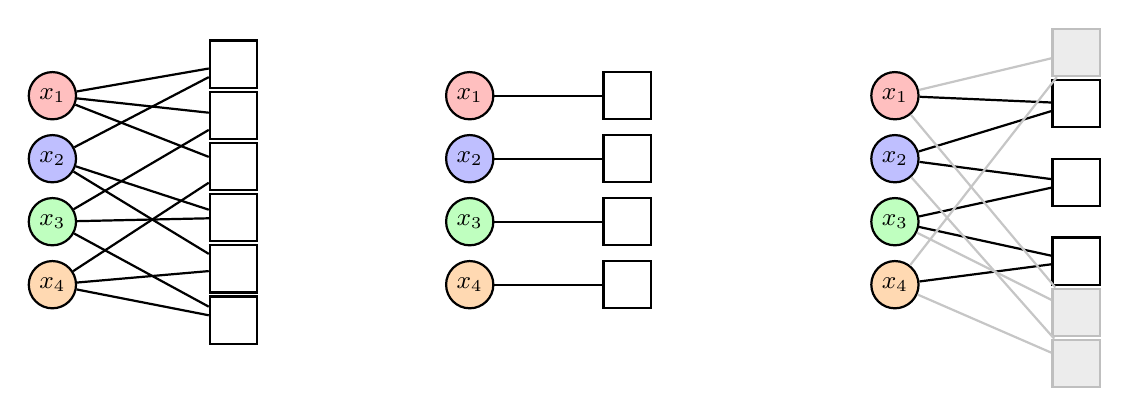
\begin{tikzpicture}[
    font=\small,
    % variable colors
    v1/.style={circle, draw, thick, fill=red!25,    minimum size=6mm, inner sep=0pt},
    v2/.style={circle, draw, thick, fill=blue!25,   minimum size=6mm, inner sep=0pt},
    v3/.style={circle, draw, thick, fill=green!25,  minimum size=6mm, inner sep=0pt},
    v4/.style={circle, draw, thick, fill=orange!30, minimum size=6mm, inner sep=0pt},
    fac/.style={rectangle, draw, thick, minimum width=6mm, minimum height=6mm, inner sep=0pt},
    facfaded/.style={rectangle, draw, thick, draw=gray!50, fill=gray!15,
        minimum width=6mm, minimum height=6mm, inner sep=0pt},
    edge/.style={draw, thick},
    faded/.style={draw, thick, gray!45},
]

% =========================================================
% Left panel: full dependency graph as 6 pairwise factors
% =========================================================
\begin{scope}[shift={(0,0)}]
% variables
\node[v1] (v1L) at (0,  1.2) {$x_1$};
\node[v2] (v2L) at (0,  0.4) {$x_2$};
\node[v3] (v3L) at (0, -0.4) {$x_3$};
\node[v4] (v4L) at (0, -1.2) {$x_4$};

% factors
\node[fac] (f12L) at (2.3,  1.60) {};
\node[fac] (f13L) at (2.3,  0.95) {};
\node[fac] (f14L) at (2.3,  0.30) {};
\node[fac] (f23L) at (2.3, -0.35) {};
\node[fac] (f24L) at (2.3, -1.00) {};
\node[fac] (f34L) at (2.3, -1.65) {};

% edges
\draw[edge] (v1L) -- (f12L);
\draw[edge] (v2L) -- (f12L);

\draw[edge] (v1L) -- (f13L);
\draw[edge] (v3L) -- (f13L);

\draw[edge] (v1L) -- (f14L);
\draw[edge] (v4L) -- (f14L);

\draw[edge] (v2L) -- (f23L);
\draw[edge] (v3L) -- (f23L);

\draw[edge] (v2L) -- (f24L);
\draw[edge] (v4L) -- (f24L);

\draw[edge] (v3L) -- (f34L);
\draw[edge] (v4L) -- (f34L);
\end{scope}

% =========================================================
% Middle panel: fully factorized (4 unary factors)
% =========================================================
\begin{scope}[shift={(5.3,0)}]
% variables
\node[v1] (v1M) at (0,  1.2) {$x_1$};
\node[v2] (v2M) at (0,  0.4) {$x_2$};
\node[v3] (v3M) at (0, -0.4) {$x_3$};
\node[v4] (v4M) at (0, -1.2) {$x_4$};

% unary factors
\node[fac] (f1M) at (2.0,  1.2) {};
\node[fac] (f2M) at (2.0,  0.4) {};
\node[fac] (f3M) at (2.0, -0.4) {};
\node[fac] (f4M) at (2.0, -1.2) {};

% edges
\draw[edge] (v1M) -- (f1M);
\draw[edge] (v2M) -- (f2M);
\draw[edge] (v3M) -- (f3M);
\draw[edge] (v4M) -- (f4M);
\end{scope}

% =========================================================
% Right panel: tree cover (3 kept pairwise factors, 3 discarded faded)
% =========================================================
\begin{scope}[shift={(10.7,0)}]
% variables
\node[v1] (v1R) at (0,  1.2) {$x_1$};
\node[v2] (v2R) at (0,  0.4) {$x_2$};
\node[v3] (v3R) at (0, -0.4) {$x_3$};
\node[v4] (v4R) at (0, -1.2) {$x_4$};

% retained tree factors
\node[fac]      (f12R) at (2.3,  1.10) {};
\node[fac]      (f23R) at (2.3,  0.10) {};
\node[fac]      (f34R) at (2.3, -0.90) {};

% discarded factors
\node[facfaded] (f14R) at (2.3,  1.75) {};
\node[facfaded] (f13R) at (2.3, -1.55) {};
\node[facfaded] (f24R) at (2.3, -2.20) {};

% retained edges
\draw[edge] (v1R) -- (f12R);
\draw[edge] (v2R) -- (f12R);

\draw[edge] (v2R) -- (f23R);
\draw[edge] (v3R) -- (f23R);

\draw[edge] (v3R) -- (f34R);
\draw[edge] (v4R) -- (f34R);

% discarded edges
\draw[faded] (v1R) -- (f14R);
\draw[faded] (v4R) -- (f14R);

\draw[faded] (v1R) -- (f13R);
\draw[faded] (v3R) -- (f13R);

\draw[faded] (v2R) -- (f24R);
\draw[faded] (v4R) -- (f24R);
\end{scope}

\end{tikzpicture}
\caption{Factor-graph representations induced by different posterior approximations. Left: the full dependency structure represented with one pairwise factor for each variable pair. Middle: a fully factorized approximation with unary factors only. Right: a tree-cover approximation retaining only the factors associated with the selected tree edges; faded factor nodes indicate discarded dependencies.}
\label{fig:chapter_5_controlled_graph_structure_dependencies}
\end{figure}

\paragraph{Controlling factor arity.}
Independently of the presence of loops, the arity of factors plays a critical role in the tractability of the inference step. To address this issue, we fix a maximum factor arity $W$ and for any constraint $c$ whose variable set $V_c$ has cardinality greater than $W$ we introduce a collection of lower-arity factors. Concretely, for each such constraint we introduce $\binom{|V_c|}{W}$ factors of arity $W$, each defined over a subset of $W$ variables. In the over-complete representation, the resulting approximation would require  $2^W \binom{|V_c|}{W}$ parameters. As shown in Figure~\ref{fig:chapter_5_controlled_graph_arity_factorgraph}, this replacement preserves part of the local interaction structure of the original constraint while reducing the parameterization cost from exponential to polynomial in the constraint size for fixed $W$.

Under this approximation, the number of parameters required to represent the contribution of the original constraint can be significantly more tractable than the original $2^{|V_c|}$ parameterization given an adequate choice of $W$.

The approximate factor graph obtained through these choices defines the family of distributions considered in the remainder of this chapter. The following section describes how features extracted from the original problem representation are mapped onto the parameters of this approximate MRF.

\begin{figure}[H]
\centering
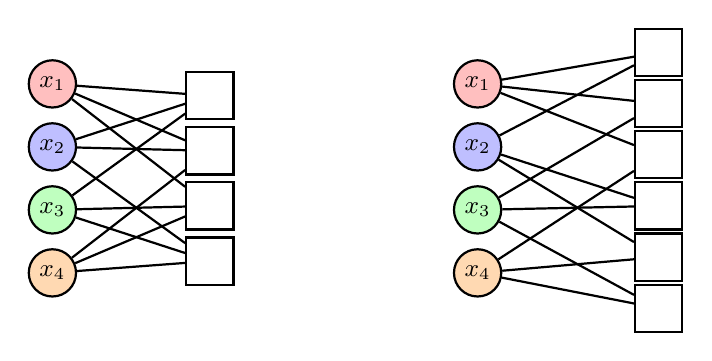
\begin{tikzpicture}[
    font=\small,
    % variable colors (consistent with previous figures)
    v1/.style={circle, draw, thick, fill=red!25,    minimum size=6mm, inner sep=0pt},
    v2/.style={circle, draw, thick, fill=blue!25,   minimum size=6mm, inner sep=0pt},
    v3/.style={circle, draw, thick, fill=green!25,  minimum size=6mm, inner sep=0pt},
    v4/.style={circle, draw, thick, fill=orange!30, minimum size=6mm, inner sep=0pt},
    fac/.style={rectangle, draw, thick, minimum width=6mm, minimum height=6mm, inner sep=0pt},
    edge/.style={draw, thick},
]

% =========================================================
% Left panel: 4 factors of arity 3
% =========================================================
\begin{scope}[shift={(0,0)}]
% variables (left column)
\node[v1] (v1L) at (0,  1.2) {$x_1$};
\node[v2] (v2L) at (0,  0.4) {$x_2$};
\node[v3] (v3L) at (0, -0.4) {$x_3$};
\node[v4] (v4L) at (0, -1.2) {$x_4$};

% factors (right column)
\node[fac] (f123) at (2.0,  1.05) {};
\node[fac] (f124) at (2.0,  0.35) {};
\node[fac] (f134) at (2.0, -0.35) {};
\node[fac] (f234) at (2.0, -1.05) {};

% edges (each arity-3 factor connects to its three variables)
\draw[edge] (v1L) -- (f123);
\draw[edge] (v2L) -- (f123);
\draw[edge] (v3L) -- (f123);

\draw[edge] (v1L) -- (f124);
\draw[edge] (v2L) -- (f124);
\draw[edge] (v4L) -- (f124);

\draw[edge] (v1L) -- (f134);
\draw[edge] (v3L) -- (f134);
\draw[edge] (v4L) -- (f134);

\draw[edge] (v2L) -- (f234);
\draw[edge] (v3L) -- (f234);
\draw[edge] (v4L) -- (f234);

%\node[align=center] at (1.0, 1.9) {Approximation with\\four arity-$3$ factors};
\end{scope}

% =========================================================
% Right panel: 6 factors of arity 2 (stacked with extra padding)
% =========================================================
\begin{scope}[shift={(5.4,0)}]
% variables (left column)
\node[v1] (v1R) at (0,  1.2) {$x_1$};
\node[v2] (v2R) at (0,  0.4) {$x_2$};
\node[v3] (v3R) at (0, -0.4) {$x_3$};
\node[v4] (v4R) at (0, -1.2) {$x_4$};

% factors stacked on the right (increased vertical spacing)
% spacing here is 0.65 between consecutive factor nodes
\node[fac] (f12) at (2.3,  1.60) {};
\node[fac] (f13) at (2.3,  0.95) {};
\node[fac] (f14) at (2.3,  0.30) {};
\node[fac] (f23) at (2.3, -0.35) {};
\node[fac] (f24) at (2.3, -1.00) {};
\node[fac] (f34) at (2.3, -1.65) {};

% edges (each factor connects to its two variables)
\draw[edge] (v1R) -- (f12);
\draw[edge] (v2R) -- (f12);

\draw[edge] (v1R) -- (f13);
\draw[edge] (v3R) -- (f13);

\draw[edge] (v1R) -- (f14);
\draw[edge] (v4R) -- (f14);

\draw[edge] (v2R) -- (f23);
\draw[edge] (v3R) -- (f23);

\draw[edge] (v2R) -- (f24);
\draw[edge] (v4R) -- (f24);

\draw[edge] (v3R) -- (f34);
\draw[edge] (v4R) -- (f34);

%\node[align=center] at (1.15, 1.9) {Approximation with\\six arity-$2$ factors};
\end{scope}

\end{tikzpicture}
\caption{Factor-graph view of arity control for posterior approximations.
Left: an approximation using four factors of arity $3$ (one per triple subset of variables).
Right: an approximation using six pairwise factors (one per variable pair).}
\label{fig:chapter_5_controlled_graph_arity_factorgraph}
\end{figure}


\subsection{Feature-to-Factor Mapping}

Having fixed the structure of the approximate MRF through the choice of an approximate factor graph, we now describe how its parameters are obtained from the input problem instance. The proposed approach follows an amortized inference paradigm: features are first extracted from a graph representation of the ILP using a graph neural network, and are then mapped to the parameters of the approximate MRF through a learned \emph{feature-to-factor mapping} operator.

We assume that a GNN has been applied to the variable--constraint bipartite representation $\VCGFULL$ of the problem, producing embeddings
\begin{equation}
\EMB^{(T)} = \bigl( \EMB^{(T)}_u \bigr)_{u \in \VCGV \cup \VCGC}, \qquad \EMB^{(T)}_u \in \mathbb{R}^d,
\end{equation}
where $\VCGV$ denotes the set of variables, $\VCGC$ the set of constraints, and $T$ the number of message-passing layers. These embeddings encode both local information and contextual interactions induced by the problem structure.

The role of the feature-to-factor mapping is to transform these embeddings into parameters of an approximate MRF defined on a factor graph $\FGFULL$ whose structure has been fixed, as described previously.

\paragraph{Precedence graph.}
The mapping from original features to the approximate MRF is guided by a dependency structure formalized through a directed bipartite graph, which we call the precedence graph and denote by $P$. This mapping specifies, for each variable or factor in the approximate MRF, which embeddings from the original problem representation it may depend on.

Formally, we define a bipartite directed graph
\begin{equation*}
\PRECG = (\PRECV \cup \FACTORSET, \PRECE),
\end{equation*}

where $\PRECV = \VCGV \cup \VCGC$ are nodes of the variable-constraint representation and $\FACTORSET$ are factors of the approximate factor graph. Note that since the variables in the original graph and the approximate factor graph are identical, only factor nodes require an explicit learned mapping. Variable node embeddings are mapped one-to-one. An edge $(u, \FACTOR) \in \PRECE$ indicates that the embedding of $u \in \PRECV$ may be used to parameterize factor $\FACTOR \in \FACTORSET$. For each factor $\FACTOR$, we denote by $N(\FACTOR) \subseteq \PRECV$ its predecessors in $\PRECG$. In practice, a dependency $(u,\FACTOR)$ is introduced whenever the set of variables associated with $u$ intersects non-trivially with the scope of $\FACTOR$; i.e. if $u$ is a variable node that belongs to the scope of factor $\FACTOR$, or if the scope of $\FACTOR$ and of the constraint represented by $u$ coincide in some variables. Figure~\ref{fig:chapter_5_factor_graph_precedence} shows that each factor of the approximate MRF receives information only from variables and constraints in the original bipartite graph whose scopes overlap with its own. For each target factor
$\FACTOR \in \FACTORSET$, we define:
\begin{itemize}
    \item a set of variable dependencies $\mathcal N_V(\FACTOR) = N(\FACTOR) \cap \VCGV$,
    \item a set of constraint dependencies $\mathcal N_C(\FACTOR) = N(\FACTOR) \cap \VCGC$.
\end{itemize}

\begin{figure}[H]
\centering
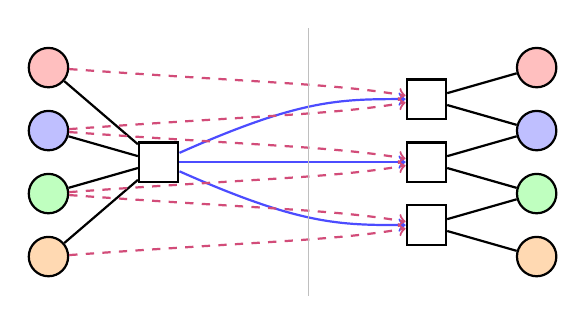
\begin{tikzpicture}[
    font=\small,
    % variable colors (consistent left/right)
    v1/.style={circle, draw, thick, fill=red!25,    minimum size=5mm, inner sep=0pt},
    v2/.style={circle, draw, thick, fill=blue!25,   minimum size=5mm, inner sep=0pt},
    v3/.style={circle, draw, thick, fill=green!25,  minimum size=5mm, inner sep=0pt},
    v4/.style={circle, draw, thick, fill=orange!30, minimum size=5mm, inner sep=0pt},
    fac/.style={rectangle, draw, thick, minimum size=5mm, inner sep=0pt},
    edge/.style={draw, thick},
    pred/.style={->, thick, draw=blue!70},
    map/.style={->, thick, dashed, draw=purple!70},
]

% -------------------------
% Left factor graph (high arity)
% -------------------------
\node[v1] (v1L) at (0,  1.2) {};
\node[v2] (v2L) at (0,  0.4) {};
\node[v3] (v3L) at (0, -0.4) {};
\node[v4] (v4L) at (0, -1.2) {};

\node[fac] (fHL) at (1.4, 0) {};

\foreach \v in {v1L,v2L,v3L,v4L}{
  \draw[edge] (\v) -- (fHL);
}

% -------------------------
% Right factor graph (low arity)
% -------------------------
\node[v1] (v1R) at (6.2,  1.2) {};
\node[v2] (v2R) at (6.2,  0.4) {};
\node[v3] (v3R) at (6.2, -0.4) {};
\node[v4] (v4R) at (6.2, -1.2) {};

\node[fac] (f12R) at (4.8,  0.8) {};
\node[fac] (f23R) at (4.8,  0.0) {};
\node[fac] (f34R) at (4.8, -0.8) {};

\draw[edge] (f12R) -- (v1R);
\draw[edge] (f12R) -- (v2R);

\draw[edge] (f23R) -- (v2R);
\draw[edge] (f23R) -- (v3R);

\draw[edge] (f34R) -- (v3R);
\draw[edge] (f34R) -- (v4R);

% -------------------------
% Precedence graph edges (colored, oriented)
% -------------------------
\draw[pred] (fHL) .. controls (3.2,  0.8) and (3.7,  0.8) .. (f12R);
\draw[pred] (fHL) .. controls (3.2,  0.0) and (3.7,  0.0) .. (f23R);
\draw[pred] (fHL) .. controls (3.2, -0.8) and (3.7, -0.8) .. (f34R);

% -------------------------
% Variable-to-factor mapping edges (dashed, oriented)
% -------------------------
\draw[map] (v1L) .. controls (2.8,  1.0) and (3.6,  1.0) .. (f12R);
\draw[map] (v2L) .. controls (2.8,  0.6) and (3.6,  0.6) .. (f12R);

\draw[map] (v2L) .. controls (2.8,  0.2) and (3.6,  0.2) .. (f23R);
\draw[map] (v3L) .. controls (2.8, -0.2) and (3.6, -0.2) .. (f23R);

\draw[map] (v3L) .. controls (2.8, -0.6) and (3.6, -0.6) .. (f34R);
\draw[map] (v4L) .. controls (2.8, -1.0) and (3.6, -1.0) .. (f34R);

% optional separator
\draw[draw=black!25] (3.3,1.7) -- (3.3,-1.7);

\end{tikzpicture}
\caption{Illustration of factor arity reduction.
Left: a single high-arity factor connected to four variables.
Right: a factor graph with only low-arity (pairwise) factors over the same variables.
Variable nodes share the same color across both graphs.
Colored arrows indicate \emph{precedence graph edges}, while dashed arrows indicate variable-to-factor mappings for pairwise factors sharing the same variables.}
\label{fig:chapter_5_factor_graph_precedence}
\end{figure}


The precedence graph is fully determined by the choice of the approximate factor graph and does not attempt to reconstruct the original high-arity constraints. Instead, it constrains information flow from the original representation to the approximate MRF.

\paragraph{Mapping features to the approximate factor graph.}
\label{sec:feature_factor_mapping}
The feature-to-factor mapping is defined independently for variables and factors of the approximate MRF.

Variables are shared between the original and approximate graphs, and their embeddings are passed through unchanged:
\begin{equation}
\EMB'_v = \EMB^{(T)}_v, \qquad \forall v \in \VCGV.
\end{equation}

For each factor $\FACTOR \in \FACTORSET$, we construct a factor embedding $\EMB'_{\FACTOR}$ by aggregating the embeddings of its dependency neighborhood:
\begin{equation}
\EMB'_{\FACTOR} =
\operatorname*{F2F}_{u \in N(\FACTOR)}
\EMB^{(T)}_u,
\qquad \forall \FACTOR \in \FACTORSET,
\end{equation}
where $\operatorname*{F2F}$ is an operator over the set of dependent embeddings, which may range from simple pooling functions (e.g., sum, mean, or max) to learned aggregation mechanisms. In its simplest variant, F2F is permutation-invariant, but this is not the case for all variants explored in the experimental section. Learned aggregation mechanisms are described in the experimental section. This aggregation step yields a fixed-dimensional representation regardless of the size of $N(\FACTOR)$.

\paragraph{Parameter prediction head.}
The parameters of the approximate MRF are obtained by applying a learned prediction head to the factor embeddings. For each factor $\FACTOR \in \FACTORSET$ of arity $|\FACTOR|$, we define
\begin{equation}
\EPARAM_{\FACTOR} = \MLP_{|\FACTOR|}\!\left( h'_{\FACTOR} \right),
\end{equation}
where $\MLP_{|\FACTOR|} : \R^d \rightarrow \R^{2^{|\FACTOR|}}$ is a multi-layer perceptron whose output dimension matches the size of the over-complete canonical parameterization for factors of that arity (see Chapter~\ref{chapter:3_differentiable_mrf_inference_for_BILPs}).

This formulation makes explicit the separation between the structure of the approximate MRF, which is fixed, and its parameterization, which is learned. Fully factorized distributions are recovered as a special case in which each factor depends only on a single variable embedding, while higher-arity factors allow the model to capture limited dependencies between variables without sacrificing tractability.

\section{Experiments}
\label{sec:chapter_5_experiments}

We now present an empirical evaluation of the proposed feature-to-factor mapping framework. Unless stated otherwise, the experimental setup closely follows that of the previous chapter. In particular, we reuse the same graph neural network architecture, hidden dimension, number of message-passing layers, optimization procedure, and training protocol. This allows us to isolate the effect of introducing structured approximate MRFs from other architectural choices.

The experiments in this section focus on evaluating the impact of the chosen approximate factor graph and of the feature-to-factor mapping on the quality of the learned distribution. We consider MRFs defined by tree-structured and pairwise factor graphs, which represent two tractable yet increasingly expressive families. In all cases, the structure of the approximate factor graph is fixed, and only its parameters are learned through the mapping described in the previous section.

Training is capped at 20 hours per model. For each configuration, three models are trained with different random seeds, and reported results are averaged across these runs. Evaluation is performed on 500 instances held out from training.

\paragraph{Training objective}
In the previous chapter, training was performed by minimizing a sum of factor-wise marginal cross-entropies between the predicted and ground-truth marginals. While this objective is natural when working with the full factor graph, we found it to be ill-suited for structured approximations with small factor arity. In particular, when using pairwise approximations, aggregating cross-entropies at the factor level leads to a strong bias towards locally consistent but globally degenerate solutions, resulting in a collapse of the learned distribution onto a small number of modes.

To mitigate this effect, the experiments reported in this section use a variable-level marginal cross-entropy loss. Concretely, training is performed by comparing the predicted unary marginals of the approximate MRF with ground-truth variable marginals, regardless of the factorization used internally by the model. This objective encourages the model to preserve meaningful uncertainty at the variable level while allowing pairwise and tree-structured factors to capture dependencies implicitly through inference.

Let $\XVEC=(\XVEC_v)_{v\in \VCGV}$ denote the binary decision variables and let $\MARGINAL_x = (\MARGINAL_v)_{v\in \VCGV}$ be the vector of unary marginals produced by the inference procedure, where
\[
\MARGINAL_v \;\triangleq\; \mathbb{P}_{p_{\EPARAM'}}(\XVEC_v=1).
\]
The marginals $\MARGINAL_{\XVEC}$ are computed by running loopy belief propagation on the chosen approximate factor graph. Let $\MARGINAL^{\star}=(\MARGINAL^{\star}_v)_{v\in\VCGV}$ denote the target unary marginals obtained from the reference solution distribution used for supervision.

We train the model by minimizing a variable-level cross-entropy between the predicted and target unary marginals:
\begin{equation}
\mathcal{L}_{\mathrm{var}}(\EPARAM')
\;=\;
-\sum_{v\in \VCGV}
\Bigl[
\MARGINAL^{\star}_v \log \MARGINAL_v
+
(1-\MARGINAL^{\star}_v)\log(1-\MARGINAL_v)
\Bigr],
\label{eq:var_ce_loss}
\end{equation}
where $\MARGINAL=\MARGINAL_{\XVEC}(\EPARAM')$ denotes the unary marginals returned by LBP on the approximate MRF parameterized by $\EPARAM'$.

The first set of results evaluates tree-structured and pairwise approximations under this training objective. More expressive feature-to-factor mappings, including attention-based and transformer-based variants, are introduced and analyzed in subsequent experiments.

\paragraph{Training data}
Consistent with the scope introduced at the beginning of the chapter, all experiments in this section are conducted on instances of the Set Covering problem. We focus on this problem class because it allows fine-grained control over the arity of constraint factors: by controlling how many sets cover each element, we directly control the size of the corresponding MRF factor. This makes SC particularly well suited for evaluating approximations with bounded factor sizes. Moreover, SC instances naturally give rise to high-arity constraints, which directly stress the limitations of over-complete canonical MRF parameterizations.

We consider three datasets. First, we reuse the two datasets with small constraint arity introduced in the previous chapter, on which the full factor graph can be represented explicitly. These datasets allow for a direct comparison between exact and approximate MRF parameterizations. Second, we introduce a new synthetic dataset specifically designed to evaluate the scalability of the proposed approach. Instances in this dataset contain constraints of arity $15$, with the total number of variables and constraints ranging between $150$ and $300$. This setting lies well beyond the regime in which explicit high-arity factor parameterizations are tractable, and therefore provides a controlled testbed for evaluating structured approximate MRFs. A description of the datasets used in this chapter is given in Table~\ref{tab:f2f_dataset_identifiers}.

\begin{table}[htbp]

\centering

\resizebox{\linewidth}{!}{
\begin{tabular}{lll}
\toprule
Name & Problem class & Description \\
\midrule

\textsc{SC-L}
& Set covering
& Larger SCP instances with $n\sim U[150,300]$, $m\sim U[150,300]$, $k=15$. \\

\textsc{MIS-L}
& Maximum independent set
& Larger MIS instances with $n\sim U[700,800]$, $p=0.15$. \\
\bottomrule
\end{tabular}}

\caption{Dataset identifiers used throughout the experimental section.}
\label{tab:f2f_dataset_identifiers}
\end{table}

\subsection{Feature-to-Factor Mapping Variants}
Here we present the variants of the feature-to-factor mapping implementations that will be tested in experiments. The variants are ordered by increasing complexity and capacity to distinguish information belonging to constraints and variable nodes. After constructing an approximate factor graph, the embeddings corresponding to a particular constraint may be involved in the construction of multiple factor embeddings but may contribute differently to each of these factors. We start by trying a simple implementation of the mapping that does not differentiate between variable and constraint embeddings, we then implement a model that explicitly separates the input between variable and constraint information and add an attention mechanism to adaptively strengthen the contribution of constraint embeddings of particular importance (learned by the model), finally we propose a transformer network layer to perform the mapping. 

\begin{table}[H]
\centering
\small
\begin{tabular}{p{2.3cm} p{3.2cm} p{7.8cm}}
\toprule
\textbf{Variant} & \textbf{Mechanism} & \textbf{Purpose} \\
\midrule
F2F-MAX & Element-wise max aggregation over all predecessors & Baseline mapping with minimal inductive bias and low capacity. \\
F2F-SEP & Explicit separation of variable and constraint embeddings & Preserve the semantic distinction between variable-level and constraint-level information. \\
F2F-ATT & Learned attention over predecessor constraints & Select the most relevant constraints for constructing each target factor embedding. \\
F2F-TRF & Transformer encoder over the dependency sequence & Model richer interactions and produce more structured factor representations. \\
\bottomrule
\end{tabular}
\caption{Summary of the feature-to-factor mapping variants.}
\label{tab:f2f_mapping_variants_compact}
\end{table}


\subsubsection{Simple Aggregation}
For both tree and pairwise approximations, the feature-to-factor mapping follows the generic formulation described in Section~\ref{sec:feature_factor_mapping}, with a simple aggregation operator. Concretely, for each factor $\FACTOR$ in the approximate graph, the corresponding factor embedding is obtained as
\begin{equation*}
\EMB'_{\FACTOR} = \max_{u \in N(\FACTOR)} h^{(T)}_u,
\end{equation*}
where the maximum is taken element-wise over the embeddings of the dependency neighborhood defined by the precedence graph. The resulting factor embedding is then passed through an arity-specific parameter prediction head to produce the parameters of the approximate MRF.

This aggregation strategy is permutation-invariant and computationally inexpensive, and makes minimal assumptions about the relative importance of the dependent embeddings. While such a simple operator may discard fine-grained information, it provides a strong baseline that allows us to isolate the effect of the MRF structure from that of the mapping architecture. Figure~\ref{fig:chapter_5_structure_prediction_simple_aggregation_mapping_figure} illustrates the F2F-MAX mapping, in which all predecessor embeddings are aggregated by a simple element-wise max operation before parameter prediction.

% Preamble:
% \usepackage{tikz}
% \usetikzlibrary{arrows.meta,positioning,fit,calc,backgrounds}

\begin{figure}[H]
\centering
\begin{tikzpicture}[
    >=Latex,
    font=\small,
    every path/.style={line width=0.9pt},
    vec/.style={draw, rounded corners=1pt, minimum width=5mm, minimum height=10mm, inner sep=0pt},
    vvec/.style={draw, rounded corners=1pt, minimum width=5mm, minimum height=10mm, inner sep=0pt, fill=green!20},
    cvec/.style={draw, rounded corners=1pt, minimum width=5mm, minimum height=10mm, inner sep=0pt, fill=blue!20},
    tiny/.style={font=\scriptsize},
    lbl/.style={font=\small}
]

% =========================================================
% Left: input set of embeddings
% =========================================================
\begin{scope}[xshift=0cm]

\node[vvec] (h1) at (0,1.8) {$h_i$};
\node[vvec] (h2) at (0,0.75) {$h_j$};
\node[cvec] (h3) at (0,-0.3) {$h_c$};

% dashed grouping box
\node[draw,dashed,rounded corners=3pt,inner sep=5pt,fit=(h1)(h2)(h3)] (ingroup) {};

\end{scope}

% arrow to matrix
\draw[->] (0.9,0.7) -- (2.0,0.7);

% =========================================================
% Middle: stacked coordinates / pooling picture
% =========================================================
\begin{scope}[xshift=2.8cm,yshift=0.2cm]

% outer matrix box
\draw[rounded corners=3pt] (-0.2,2.5) rectangle (2.9,-1.4);

% first row
\node[tiny] (hi1) at (0.45,1.7) {$h_i^{(1)}$};
\node[tiny] (hj1) at (1.35,1.7) {$h_j^{(1)}$};
\node[tiny] (hc1) at (2.25,1.7) {$h_c^{(1)}$};

% second row
\node[tiny] at (0.45,0.95) {$h_i^{(2)}$};
\node[tiny] at (1.35,0.95) {$h_j^{(2)}$};
\node[tiny] at (2.25,0.95) {$h_j^{(2)}$};

% dots
\node[tiny] at (0.45,0.25) {$\vdots$};
\node[tiny] at (1.35,0.25) {$\vdots$};
\node[tiny] at (2.25,0.25) {$\vdots$};

% last row
\node[tiny] at (0.45,-0.65) {$h_i^{(d)}$};
\node[tiny] at (1.35,-0.65) {$h_j^{(d)}$};
\node[tiny] at (2.25,-0.65) {$h_{|N(\alpha)|}^{(d)}$};

% dashed highlight on one column
\begin{scope}[on background layer]
\node[
  draw,
  dashed,
  rounded corners=1pt,
  inner sep=1pt,
  fill=yellow!20,
  fit=(hi1)(hj1)(hc1)
] (ingroup_o) {};
\end{scope}

\end{scope}

% arrow to matrix
\draw[->] (6.4,0.7) -- (7.5,0.7);

% =========================================================
% Right: output embedding
% =========================================================
\begin{scope}[xshift=6.9cm]

\node[tiny] (ha1) at (2,1.8) {$h_{\alpha}^{(1)}$};
\node[tiny] (ha2) at (2,0.75) {$\vdots$};
\node[tiny] (ha3) at (2,-0.3) {$h_{\alpha}^{(d)}$};

\begin{scope}[on background layer]
\node[
  draw,
  rounded corners=3pt,
  inner sep=1pt,
  fill=purple!15,
  fit=(ha1)(ha2)(ha3)
] (ingroup_a) {};
\end{scope}

\node[draw,rounded corners=3pt,inner sep=1pt,fit=(ha1)(ha2)(ha3)] (ingroup_a) {};

\node[tiny,right=3mm of ha1] {$ = \square \left( h_i^{(1)}, h_j^{(1)}, h_c^{(1)} \right)$};
\node[tiny,right=3mm of ha3] {$ = \square \left( h_i^{(d)}, h_j^{(d)}, h_c^{(d)} \right)$};

\end{scope}

\end{tikzpicture}
\caption{Permutation-invariant construction of the factor embedding \(h_{\alpha}\) from the embeddings of the nodes in $N(\alpha) = \{ i,j,c \}$, illustrated here with coordinate-wise aggregation $\square$.}
\label{fig:chapter_5_structure_prediction_simple_aggregation_mapping_figure}
\end{figure}

\subsubsection{Separating variable / constraint features}
This variant aims to identify the degree of importance of the variable embeddings versus the constraint information. In this model the only difference is constructing the parameter head predictors by explicitly splitting the input of the MLP into a vector of variable embeddings and a vector of constraint embeddings. We test the \emph{variable-only} model (F2F-VAR) in which constraint embeddings are simply not passed to the model.

The parameter prediction head input given by $\square_{v \in N(\FACTOR')} h_v$ may be garbled, i.e. aggregating all features for variables and constraints alike leads to a loss of information. Factor embeddings are defined
\begin{equation}
    \EMB'_{\FACTOR} = \left[ \EMB^{(T)}_{i_1},...,\EMB^{(T)}_{i_{|\FACTOR|}}, \underset{c \in \mathcal{N}_C(\FACTOR)}{\square} \EMB^{(T)}_{c} \right] \in \R^{(|\FACTOR| + 1) d}
\end{equation}
with $\square $ still defined as an aggregation function (taken as the $\max$ operator in experiments) and $(i_1,...,i_{|\FACTOR|})$ is an ordering of the variables in the scope of $\FACTOR$. The input dimensions of the parameter prediction heads are adapted to the new factor embedding shape $\EMB'_{\FACTOR} \in \R^{(|\FACTOR|+1) d}$. Figure~\ref{fig:chapter_5_structure_prediction_var_constr_separation_mapping_figure} illustrates how F2F-SEP separates variable embeddings from aggregated constraint information before concatenating them into the factor representation.

We expect this separation to improve the quality of the predicted factor parameters by preventing variable and constraint information from being mixed too early, thereby allowing the prediction head to exploit their distinct semantic roles more effectively.

\begin{figure}[H]
\centering
\begin{tikzpicture}[
    >=Latex,
    font=\small,
    every path/.style={line width=0.9pt},
    vec/.style={draw, rounded corners=1pt, minimum width=6mm, minimum height=10mm, inner sep=1pt},
    vvec/.style={draw, rounded corners=1pt, minimum width=6mm, minimum height=10mm, inner sep=1pt, fill=green!20},
    cvec/.style={draw, rounded corners=1pt, minimum width=6mm, minimum height=10mm, inner sep=1pt, fill=blue!20},
    ovec/.style={draw, rounded corners=1pt, minimum width=6mm, minimum height=10mm, inner sep=1pt, fill=magenta!20},
    tiny/.style={font=\scriptsize},
    lbl/.style={font=\small}
]

% =========================================================
% Left: separate variable embeddings
% =========================================================
\begin{scope}[xshift=0cm]

\node[vvec] (hi) at (0,1.2) {$h_i$};
\node[vvec] (hj) at (0,0.0) {$h_j$};

\node[cvec] (hc1) at (0,-1.2) {$h_{c_1}$};
\node[cvec] (hc2) at (0,-2.4) {$h_{c_2}$};

\node[fit=(hc1)(hc2),inner sep=2pt] (hc_group) {};

\draw[
    decorate,
    decoration={brace, amplitude=6pt}
]
([xshift=6pt]hc_group.north east) -- ([xshift=6pt]hc_group.south east)
node[midway, left=6pt] {};

\node[draw,dashed,rounded corners=3pt,inner sep=5pt,fit=(hi)(hj)(hc1)(hc2)] {};

\end{scope}


% arrow from constraint set to aggregation


% =========================================================
% Middle: aggregation of constraint features only
% =========================================================
\begin{scope}[xshift=3.3cm,yshift=-2.5cm]
\draw[->] (-2.2,0.75) -- (-1.1,0.75);

% outer matrix box
\draw[rounded corners=3pt] (-0.2,2.5) rectangle (2.1,-1.4);

% first row
\node[tiny] (ha11) at (0.45,1.7) {$h_{c_1}^{(1)}$};
\node[tiny] (ha21) at (1.35,1.7) {$h_{c_2}^{(1)}$};

% second row
\node[tiny] at (0.45,0.95) {$h_{c_1}^{(2)}$};
\node[tiny] at (1.35,0.95) {$h_{c_2}^{(2)}$};

% dots
\node[tiny] at (0.45,0.25) {$\vdots$};
\node[tiny] at (1.35,0.25) {$\vdots$};

% last row
\node[tiny] at (0.45,-0.65) {$h_{c_1}^{(d)}$};
\node[tiny] at (1.35,-0.65) {$h_{c_2}^{(d)}$};

% dashed highlight on one coordinate row? no, keep column like previous
\begin{scope}[on background layer]
\node[
  draw,
  dashed,
  rounded corners=1pt,
  inner sep=1pt,
  fill=yellow!20,
  fit=(ha11)(ha21)
] {};
\end{scope}

\draw[->] (2.9,0.75) -- (4.0,0.75);

\end{scope}

% arrow to aggregated constraint vector


% =========================================================
% Right: separate inputs to prediction head
% =========================================================
\begin{scope}[xshift=9.7cm]

\node[vvec] (ohi) at (0,0.8) {$h_i$};
\node[vvec] (ohj) at (0,-0.3) {$h_j$};

\node[ovec] (ohc1) at (0,-1.6) {$\underset{c \in \mathcal N(\alpha)\cap C}{\square} h_c$};

\begin{scope}[on background layer]
\node[
  draw,dashed,
  rounded corners=3pt,
  inner sep=4pt,
  %fill=purple!15,
  fit=(ohi)(ohj)(ohc1)
] {};
\end{scope}

%\node[draw,rounded corners=3pt,inner sep=4pt,fit=(ohi)(ohj)(ohc1)] {};

\end{scope}

\end{tikzpicture}
\caption{Separating variable and constraint features in the parameter prediction head. Variable embeddings \(h_i\) and \(h_j\) are kept as distinct inputs, while only neighboring constraint embeddings are aggregated coordinate-wise into a last input.}
\label{fig:chapter_5_structure_prediction_var_constr_separation_mapping_figure}
\end{figure}

\subsubsection{Mapping with Attention}
The previous proposal still aggregates over all constraint embeddings, disregarding their importance level. We propose to add an attention prediction head to attribute more importance to certain constraints over others. Factor embeddings are constructed :
\begin{equation}
    \EMB'_{\FACTOR} = \left[ \EMB^{(T)}_{i_1},...,\EMB^{(T)}_{i_{|\FACTOR|}}, \EMB^c_{\FACTOR} \right] \in \R^{(|\FACTOR| + 1) d}
\end{equation}
with $\EMB^c_{\FACTOR}$ an embedding representing the constraints upon which factor $\FACTOR$ depends, and is defined
\begin{align}
    \EMB^c_{\FACTOR} &= \sum\limits_{c \in \mathcal{N}_C(\FACTOR)} \beta_{\FACTOR,c} \EMB^{(T)}_{c}
\end{align}
with attention 
\begin{align}
    \hat{\beta}_{\FACTOR,c} &=  \MLP \left(  \EMB^{(T)}_{i_1},...,\EMB^{(T)}_{i_{|\FACTOR|}}, \EMB^{(T)}_{c} \right) \\
    \beta_{\FACTOR,c} &= \frac{\exp \hat{\beta}_{\FACTOR,c}}{\sum\limits_{c \in \mathcal{N}_C(\FACTOR)} \exp \hat{\beta}_{\FACTOR,c}}
\end{align}

Figure~\ref{fig:chapter_5_structure_prediction_constr_attention_mapping_figure} shows the F2F-ATT architecture, where the contribution of each predecessor constraint embedding is weighted by a learned attention score before being incorporated into the factor embedding.

This variant is expected to improve over F2F-SEP when not all predecessor constraints are equally informative for a given target factor, as the attention mechanism allows the model to identify and emphasize the most relevant constraints while down-weighting less useful ones.

\begin{figure}[H]
\centering
\begin{tikzpicture}[
    >=Latex,
    font=\small,
    every path/.style={line width=0.9pt},
    vec/.style={draw, rounded corners=1pt, minimum width=6mm, minimum height=10mm, inner sep=1pt},
    vvec/.style={draw, rounded corners=1pt, minimum width=6mm, minimum height=10mm, inner sep=1pt, fill=green!20},
    cvec/.style={draw, rounded corners=1pt, minimum width=6mm, minimum height=10mm, inner sep=1pt, fill=blue!20},
    ovec/.style={draw, rounded corners=1pt, minimum width=6mm, minimum height=10mm, inner sep=1pt, fill=magenta!20},
    tiny/.style={font=\scriptsize},
    lbl/.style={font=\small}
]

% =========================================================
% Left: separate variable and constraint embeddings
% =========================================================
\begin{scope}[xshift=0cm]

\node[vvec] (hi)  at (0, 1.2) {$h_i$};
\node[vvec] (hj)  at (0, 0.0) {$h_j$};

\node[cvec] (hc1) at (0,-1.2) {$h_{c_1}$};
\node[cvec] (hc2) at (0,-2.4) {$h_{c_2}$};

\node[draw,dashed,rounded corners=3pt,inner sep=5pt,fit=(hi)(hj)(hc1)(hc2)] {};

\end{scope}

% =========================================================
% Middle: attention-weighted aggregation
% =========================================================
\begin{scope}[xshift=4.2cm]


% weights stack
\node[draw,rounded corners=2pt,fill=orange!15,minimum width=11mm,minimum height=7mm] (b1) at (1.9,-1.2) {\tiny $\beta_{ij,c_1}$};
\node[draw,rounded corners=2pt,fill=orange!15,minimum width=11mm,minimum height=7mm] (b2) at (1.9,-2.4) {\tiny $\beta_{ij,c_2}$};

% weighted sum node
\node[draw,rounded corners=3pt,fill=yellow!20,minimum width=9mm,minimum height=16mm] (sum) at (4.0,-1.8) {$\sum$};

% arrows
\draw[->] ([xshift=2mm]hc1.east) -- (b1.west);
\draw[->] ([xshift=2mm]hc2.east) -- (b2.west);

\draw[->] (b1.east) -- (sum.west |- b1.east);
\draw[->] (b2.east) -- (sum.west |- b2.east);

% aggregated constraint embedding
%\draw[->] (sum.east) -- (5.2,-1.8);
%\node[ovec] (hcagg) at (6.1,-1.8) {$h^c_{ij}$};

% from h_i
\begin{scope}[on background layer]
    \draw[->] ([xshift=2mm]hi.east) -| ([xshift=1mm]b1.north);
    \draw[->] ([xshift=2mm]hi.east) -| ([xshift=1mm]b2.north);
    \draw[->] ([xshift=2mm]hj.east) -| ([xshift=-1mm]b1.north);
    \draw[->] ([xshift=2mm]hj.east) -| ([xshift=-1mm]b2.north);
\end{scope}


\end{scope}

% =========================================================
% Right: inputs to prediction head
% =========================================================
\begin{scope}[xshift=12.0cm]

\node[vvec] (ohi) at (0, 0.8) {$h_i$};
\node[vvec] (ohj) at (0,-0.3) {$h_j$};
\node[ovec] (ohc)  at (0,-1.8) {$h^c_{ij}$};
\draw[->] (sum.east) -- ([xshift=-2mm]ohc.west);


\begin{scope}[on background layer]
\node[
  draw,dashed,
  rounded corners=3pt,
  inner sep=4pt,
  fit=(ohi)(ohj)(ohc)
] {};
\end{scope}

\end{scope}

\end{tikzpicture}
\caption{Attention-based aggregation of constraint embeddings. Variable embeddings \(h_i\) and \(h_j\) remain distinct inputs, while neighboring constraint embeddings are combined into \(h^c_{ij}\) by a weighted sum with attention coefficients \(\beta_{ij,c}\) predicted from \((h_i,h_j,h_c)\).}
\label{fig:chapter_5_structure_prediction_constr_attention_mapping_figure}
\end{figure}

\subsubsection{Transformer Mapping}
\label{sssec:chapter_5_variant_p3}

The previous mappings construct each target factor embedding independently from the features of its neighboring variables and constraints. In this proposal, we instead represent each target factor by a short input sequence and use a transformer encoder to learn interactions between the different elements of this sequence before predicting the factor parameters.


We denote by
\[
K_V = \max_{\FACTOR \in \FACTORSET} |\mathcal N_V(\FACTOR)|,
\qquad
K_C = \max_{\FACTOR \in \FACTORSET} |\mathcal N_C(\FACTOR)|,
\]
the maximum number of variable and constraint dependencies over all target factors, and define
\[
S = K_V + K_C .
\]

For each target factor $\FACTOR$, we build a sequence of length $S$ by listing first the embeddings of its dependent variables and then the embeddings of its dependent constraints, padding with null tokens whenever fewer than $K_V$ or $K_C$ elements are present. Thus, the transformer input is a tensor

$$g_0 \in \R^{|F| \times S \times d}$$

More explicitly, for each target factor $\FACTOR_m$, the slice $g_0[m,:,:]$ is of the form
\begin{equation}
g_0[m,:,:]
=
\Big[
\EMB^{(T)}_{v_1},\,
\ldots,\,
\EMB^{(T)}_{v_{|\mathcal N_V(\FACTOR_m)|}},\,
0,\ldots,0,\,
\EMB^{(T)}_{c_1},\,
\ldots,\,
\EMB^{(T)}_{c_{|\mathcal N_C(\FACTOR_m)|}},\,
0,\ldots,0
\Big],
\end{equation}
where $(v_1,\dots,v_{|\mathcal N_V(\FACTOR_m)|})$ enumerates the variable dependencies in $\mathcal N_V(\FACTOR_m)$, $(c_1,\dots,c_{|\mathcal N_C(\FACTOR_m)|})$ enumerates the constraint dependencies in $\mathcal N_C(\FACTOR_m)$, and each element of the sequence belongs to $\R^d$.

Since the number of dependencies varies across target factors, we additionally define a binary padding mask $M \in \{0,1\}^{|\FACTORSET| \times S}$, with
\begin{equation*}
M_{m,s} =
\begin{cases}
1, & \text{if token } s \text{ of target factor } \FACTOR_m \text{ corresponds to a real dependency},\\
0, & \text{if token } s \text{ is padding}.
\end{cases}
\end{equation*}

The transformer then produces a sequence of hidden representations
\begin{equation*}
g_1, g_2, \dots, g_L,
\qquad
g_\ell \in \mathbb R^{|\FACTORSET| \times S \times d},
\end{equation*}
where each layer applies self-attention over the dependency tokens of each target factor, using the mask $M$ to ignore padded positions. The embedding of factor $\FACTOR_m$ is then simply taken to be the average value of each slice along the second dimension: 
\begin{equation}
    \EMB'_{\FACTOR_m} = \frac{1}{\sum^S_{s=1} M_{m,s}} \sum\limits_{s=1}^S M_{m,s} g_{L}[m,s,:] \in \mathbb{R}^d
\end{equation}

Figure~\ref{fig:chapter_5_structure_prediction_transformer_mapping_figure} illustrates the F2F-TRF mapping, in which variable and constraint embeddings are arranged into a padded sequence and processed jointly by a transformer encoder before pooling.

The transformer-based model should outperform other variants when proper parameterization requires combining and disentangling multiple sources of variable- and constraint-level information, since self-attention can model higher-order interactions within the dependency set of each target factor.

% Preamble:
% \usepackage{tikz}
% \usetikzlibrary{arrows.meta,positioning,fit,calc,backgrounds}

\begin{figure}[H]
\centering
\resizebox{.99\linewidth}{!}{
\begin{tikzpicture}[
    >=Latex,
    font=\small,
    every path/.style={line width=0.9pt},
    vvec/.style={draw, rounded corners=1pt, minimum width=7mm, minimum height=10mm, inner sep=1pt, fill=green!20},
    cvec/.style={draw, rounded corners=1pt, minimum width=7mm, minimum height=10mm, inner sep=1pt, fill=blue!20},
    pvec/.style={draw, rounded corners=1pt, minimum width=7mm, minimum height=10mm, inner sep=1pt, fill=gray!15},
    ovec/.style={draw, rounded corners=1pt, minimum width=8mm, minimum height=10mm, inner sep=1pt, fill=magenta!20},
    tiny/.style={font=\scriptsize},
    lbl/.style={font=\small},
    block/.style={draw, rounded corners=3pt, minimum width=15mm, minimum height=10mm, align=center, fill=orange!15}
]

% =========================================================
% Left: dependency tokens for one target factor
% =========================================================
\begin{scope}[xshift=0cm]
\node[vvec] (hi) at (0,1.8) {$h_i$};
\node[vvec] (hj) at (0,0.6) {$h_j$};
\node[cvec] (hc1) at (0,-0.8) {$h_{c_1}$};
\node[cvec] (hc2) at (0,-2.0) {$h_{c_2}$};

\node[draw,dashed,rounded corners=3pt,inner sep=5pt,fit=(hi)(hj)(hc1)(hc2)] {};
%\node[lbl] at (0,-3.0) {dependencies of $\alpha'$};
\end{scope}

\draw[->] (0.8,-0.1) -- (1.9,-0.1);

% =========================================================
% Middle-left: packed tensor slice g0[m,:,:]
% =========================================================
\begin{scope}[xshift=2cm,yshift=-0.1cm]

% front face
\coordinate (A) at (0,1.5);
\coordinate (B) at (2.7,1.5);
\coordinate (C) at (2.7,-1.9);
\coordinate (D) at (0,-1.9);

% depth shift
\coordinate (s) at (0.45,0.35);

% back face
\coordinate (A2) at ($(A)+(s)$);
\coordinate (B2) at ($(B)+(s)$);
\coordinate (C2) at ($(C)+(s)$);
\coordinate (D2) at ($(D)+(s)$);

% draw parallelepiped
\fill[gray!6] (A) -- (B) -- (C) -- (D) -- cycle;
\fill[gray!10] (A) -- (A2) -- (B2) -- (B) -- cycle;
\fill[gray!14] (B) -- (B2) -- (C2) -- (C) -- cycle;

\draw (A) -- (B) -- (C) -- (D) -- cycle;
\draw (A) -- (A2) -- (B2) -- (B);
\draw (B2) -- (C2) -- (C);
%\draw[dashed] (A2) -- (D2) -- (C2);
%\draw[dashed] (D) -- (D2);


% token separators on front face
\draw (0,0.65) -- (2.7,0.65);
\draw (0,-0.20) -- (2.7,-0.20);
\draw (0,-1.05) -- (2.7,-1.05);

%\draw[dashed] (0,0.65) -- ($(0,0.65)+(s)$);
%\draw[dashed] (0,-0.20) -- ($(0,-0.20)+(s)$);
%\draw[dashed] (0,-1.05) -- ($(0,-1.05)+(s)$);

\draw (2.7,0.65) -- ($(2.7,0.65)+(s)$);
\draw (2.7,-0.20) -- ($(2.7,-0.20)+(s)$);
\draw (2.7,-1.05) -- ($(2.7,-1.05)+(s)$);


% labels inside slice
\node[tiny] at (1.05,1.08) {$h_i\in\mathbb{R}^d$};
\node[tiny] at (1.05,0.22) {$h_j\in\mathbb{R}^d$};
\node[tiny] at (1.05,-0.63) {$h_{c_1}\in\mathbb{R}^d$};
\node[tiny] at (1.05,-1.48) {$h_{c_2}\in\mathbb{R}^d$};

% \node[tiny] at (2.15,1.08) {$\in\mathbb{R}^d$};
% \node[tiny] at (2.15,0.22) {$\in\mathbb{R}^d$};
% \node[tiny] at (2.15,-0.63) {$\in\mathbb{R}^d$};
% \node[tiny] at (2.15,-1.48) {$\in\mathbb{R}^d$};

% tensor labels
\node[lbl] at (1.6,-2.75) {$g_0[m,:,:] \in \mathbb{R}^{S\times d}$};
%\node[tiny] at (3.45,-0.2) {$m$};
%\node[tiny] at (1.35,1.95) {$S$};
%\node[tiny] at (3.05,1.85) {$d$};

\end{scope}

%\draw[->] (6.2,-0.1) -- (7.2,-0.1);

% =========================================================
% Middle: transformer stack
% =========================================================
\begin{scope}[xshift=7.8cm,yshift=-0.1cm]
\node[block] (tr1) at (0,1.5) {MHA};
\node[block] (tr2) at (0,0) {FFN};
\node[block] (tr3) at (0,-1.5) {LN};

\draw[->] (-2.5,-0) -- ++(1,0) |- (tr1.west);
\draw[->] (tr1.south) -- (tr2.north);
\draw[->] (tr2.south) -- (tr3.north);
\draw[->] (tr3.east) -- ++(1.5,0) node[midway,fill=white] (tr_mid) {$g_\ell$} -- ++(0,1.5) -- ++(0.5,0);

\draw[->] (tr_mid.south) -- ++(0,-.75) -- ++(-3,0) -- ++(0,4) |- (tr1.west);

\node[lbl] at (0,-3.0) {$L$ transformer layers};
\end{scope}

% =========================================================
% Right: output tensor slice gL[m,:,:]
% =========================================================
\begin{scope}[xshift=10.6cm,yshift=-0.1cm]

% front face
\coordinate (E) at (0,1.5);
\coordinate (F) at (2.7,1.5);
\coordinate (G) at (2.7,-1.9);
\coordinate (H) at (0,-1.9);

% depth shift
\coordinate (t) at (0.45,0.35);

% back face
\coordinate (E2) at ($(E)+(t)$);
\coordinate (F2) at ($(F)+(t)$);
\coordinate (G2) at ($(G)+(t)$);
\coordinate (H2) at ($(H)+(t)$);

% draw parallelepiped
\fill[magenta!8] (E) -- (F) -- (G) -- (H) -- cycle;
\fill[magenta!12] (E) -- (E2) -- (F2) -- (F) -- cycle;
\fill[magenta!16] (F) -- (F2) -- (G2) -- (G) -- cycle;

\draw (E) -- (F) -- (G) -- (H) -- cycle;
\draw (E) -- (E2) -- (F2) -- (F);
\draw (F2) -- (G2) -- (G);
%\draw[dashed] (E2) -- (H2) -- (G2);
%\draw[dashed] (H) -- (H2);

% token separators on front face
\draw (0,0.65) -- (2.7,0.65);
\draw (0,-0.20) -- (2.7,-0.20);
\draw (0,-1.05) -- (2.7,-1.05);

\draw (2.7,0.65) -- ($(2.7,0.65)+(t)$);
\draw (2.7,-0.20) -- ($(2.7,-0.20)+(t)$);
\draw (2.7,-1.05) -- ($(2.7,-1.05)+(t)$);

% labels inside slice
\node[tiny] at (1.15,1.08) {$\tilde h_i \in \mathbb{R}^d$};
\node[tiny] at (1.15,0.22) {$\tilde h_j \in \mathbb{R}^d$};
\node[tiny] at (1.15,-0.63) {$\tilde h_{c_1} \in \mathbb{R}^d$};
\node[tiny] at (1.15,-1.48) {$\tilde h_{c_2} \in \mathbb{R}^d$};

\node[lbl] at (1.6,-2.75) {$g_L[m,:,:] \in \mathbb{R}^{S\times d}$};

\end{scope}

\draw[->] (13.8,-0.1) -- (14.6,-0.1);

\node[draw,rounded corners=3pt,fill=yellow!20,minimum width=9mm,minimum height=16mm] (sum) at (15,-0.1) {$\sum$};

% =========================================================
% Far right: pooled / selected representation
% =========================================================
\begin{scope}[xshift=15.5cm,yshift=-0.1cm]
\node[ovec] (hout) at (1,-0) {$h_{\alpha}$};
\draw[->] (sum.east) -- (hout.west);
%\node[lbl] at (0,-1.1) {factor embedding};
\end{scope}

% overall title-ish annotation
%\node[lbl] at (8.0,2.25) {$g_0 \in \mathbb{R}^{N\times S\times d} \;\longrightarrow\; g_L \in \mathbb{R}^{N\times S\times d}$};

\end{tikzpicture}}
\caption{Transformer-based feature mapping. For each target factor $\alpha'$, the embeddings of its dependent variables and constraints are packed into a tensor slice $g_0[m,:,:] \in \mathbb{R}^{S\times d}$. A stack of transformer layers produces contextualized representations $g_L[m,:,:]$, from which the factor embedding $h_{\alpha}$ is derived. Over all target factors, the full tensor has shape $g_0,g_L \in \mathbb{R}^{N\times S\times d}$.}
\label{fig:chapter_5_structure_prediction_transformer_mapping_figure}
\end{figure}

\begin{table}[H]
\centering
\small
\begin{tabular}{p{2.2cm} p{3.1cm} p{7.2cm}}
\toprule
\textbf{Label} & \textbf{Category} & \textbf{Meaning} \\
\midrule
DGN & Baseline model & Fully factorized predictor with independent variable scores and no MRF inference. \\
F2F-MAX/SEP/VAR/ATT/TRF & Mapping variant & Neural mechanism used to map GNN embeddings to factor parameters. \\
FULL & Factor graph structure & Original constraint-factor MRF; used only when the full canonical factor tables are tractable. \\
PAIR & Factor graph structure & Pairwise approximation containing only factors of arity at most two. \\
TREE & Factor graph structure & Sparse tree-structured approximation, obtained from a spanning tree of the dependency graph. \\
EGG/GD & Decoding policy & Procedures used to convert predicted marginals into feasible assignments. \\
\bottomrule
\end{tabular}
\caption{Terminology used in the experimental section. Mapping labels describe how factors are parameterized, whereas FULL, PAIR, and TREE describe which factor graph is parameterized.}
\label{tab:chapter_5_experimental_terminology}
\end{table}

\subsection{Results}
\label{subsec:chapter_5_results}

The experiments vary three conceptually distinct components: the feature-to-factor mapping, the approximate MRF structure, and the decoding policy. To avoid ambiguity, we use the following terminology throughout the section. The labels F2F-MAX, F2F-SEP, F2F-VAR, F2F-ATT, and F2F-TRF denote neural mapping architectures that convert embeddings from the original variable--constraint graph into factor parameters. In contrast, FULL, PAIR, and TREE denote the structure of the MRF being parameterized. FULL is the original constraint-factor graph and is evaluated only on low-arity instances where the canonical factor representation is tractable. PAIR is a bounded pairwise approximation, and TREE is a spanning-tree approximation of the variable-dependency graph. Finally, EGG and GD denote decoding strategies applied to the marginals returned by inference.

The first set of experiments evaluates the effect of the mapping architecture for a fixed factor-graph protocol on each dataset. The later decoding-dynamics analysis fixes the mapping to F2F-TRF and varies the factor-graph structure among FULL, PAIR, and TREE. Thus, differences between F2F variants measure the effect of parameterization capacity, whereas differences between FULL, PAIR, and TREE measure the effect of structural approximation.

As discussed previously, exact MRF parameterizations quickly become intractable as constraint arity increases. The experiments in this section evaluate how well the proposed approximate MRF constructions mitigate this limitation in practice. We focus on assessing the impact of the chosen factor graph structure and feature-to-factor mapping on the quality of the learned distributions, and analyze the trade-offs between expressivity and tractability across different approximation regimes. Table ~\ref{tab:chapter_5_scp50_results}-~\ref{tab:chapter_5_scp_n150_results} reports the performance of all considered mapping variants across the datasets of increasing constraint arity. Results are evaluated using both EGG and GD decoding.

We evaluate the five proposed variants of the feature-to-factor component under approximate factor graphs of increasing complexity. Each F2F variant is paired either with a tree-structured factor graph obtained from a minimum spanning tree of the supporting dependency graph, denoted MST, or with a bounded-arity factor graph in which every factor $\FACTOR$ satisfies $|\FACTOR|\leq k$. The arity bound controls the expressiveness and cost of the approximate MRF: larger values of $k$ allow richer local dependencies, but require larger factor tables and more expensive LBP updates.

For all instance classes, we report the performance of the fully factorized baseline, denoted DGN, which predicts independent variable scores and does not use an MRF layer. For the smaller instances, where the full canonical factor parameterization remains tractable, we also report the performance of the LMRF-LBP model from Chapter~\ref{chapter:3_differentiable_mrf_inference_for_BILPs}. This model serves as a high-expressivity reference point for assessing how much is lost when the original high-arity constraint factors are replaced by tractable approximate factor graphs.

\paragraph{On the choice of factor graph approximation}

On the two lower-arity datasets (Tables~\ref{tab:chapter_5_scp50_results} and \ref{tab:chapter_5_scp_n120_results}), the choice of factor graph approximation has a clear and consistent impact on solution quality. As the maximum factor arity increases, the optimality gap decreases across all mapping variants. For instance, on the $(n=50)$ dataset, moving from pairwise models ($|\FACTOR| \leq 2$) to higher-arity approximations ($|\FACTOR| \leq 4$) reduces the GD gap from approximately $2.9\%$ to $2.0\%$ for F2F-MAX, and from $3.3\%$ to $2.5\%$ for F2F-SEP. A similar trend is observed for F2F-ATT and F2F-TRF, indicating that increasing factor arity consistently improves performance.

This behavior is expected: higher-arity factors allow the approximate MRF to better capture the combinatorial structure of the constraints, leading to more accurate local representations of feasibility. In contrast, low-arity approximations break higher-order dependencies into independent or weakly coupled interactions, which limits the model’s ability to represent valid joint configurations.

The difference between the two decoding strategies further highlights the role of modeled dependencies. When using EGG, improvements from increasing factor arity remain moderate, as decisions are made based solely on the initial marginals. In contrast, the GD procedure consistently yields substantially lower optimality gaps. For example, on the SC-S dataset with $|\FACTOR| \leq 4$, GD improves over greedy by more than $3$ percentage points across most models.

This gap can be attributed to the ability of GD to exploit the learned dependencies: as variables are fixed, marginals are recomputed, allowing the model to propagate constraints and refine its predictions. As a result, the marginals become increasingly informative throughout the decoding process, effectively guiding the search toward more feasible and higher-quality solutions.

However, this comes at a significant computational cost, as inference must be rerun after each variable assignment. This highlights a fundamental trade-off: while richer factor graph approximations improve solution quality, their benefits are most pronounced when combined with iterative inference procedures such as GD.

\paragraph{On the choice of feature-to-factor mapping}
Having established that the structure of the approximate factor graph strongly influences performance, we now examine the contribution of the feature-to-factor mapping itself. Overall, increasing the expressivity of the mapping leads to consistent but moderate improvements, provided that the underlying factor graph is sufficiently informative. Comparing F2F-MAX and F2F-SEP highlights the importance of explicitly separating variable and constraint information: while both models rely on simple aggregation mechanisms, F2F-SEP typically achieves slightly improved performance, indicating that preserving this structural distinction is beneficial. In contrast, the F2F-VAR variant, which discards constraint embeddings entirely, consistently degrades performance, confirming that constraint-level information is essential for accurately parameterizing the approximate MRF.

Moving to more expressive mappings, F2F-ATT introduces attention over constraint embeddings, allowing the model to selectively weight the contribution of different constraints. This results in more stable behavior and modest improvements across most settings, suggesting that not all constraints contribute equally to the parameterization of a given factor. Finally, the transformer-based mapping F2F-TRF further increases modeling capacity by allowing interactions between all dependency embeddings. While this additional flexibility can yield further gains—particularly in intermediate regimes—it does not lead to uniformly large improvements over F2F-ATT, indicating that the main benefit comes from identifying relevant dependencies rather than modeling complex higher-order interactions between them.

Taken together, these results suggest that while improving the mapping function is beneficial, its impact remains secondary to that of the factor graph structure. In particular, more expressive mappings are most effective when combined with sufficiently rich factor graph approximations, and cannot fully compensate for overly restrictive structural choices.

\paragraph{Failure modes on high-arity instances}
The results on the largest dataset (Table~\ref{tab:chapter_5_scp_n150_results}) reveal important limitations of the proposed approximation scheme. In this regime, constraints involve a large number of variables, and the reduction to low-arity factors leads to unstable behavior during training, with some seeds consistently failing to converge. This suggests that decomposing high-arity constraints into collections of small factors is insufficient to faithfully capture the underlying dependencies between variables. In particular, the resulting approximate MRF appears unable to represent the global interactions induced by large constraints, leading to degraded performance and increased variance across runs. These observations highlight a fundamental limitation of fixed low-arity approximations in highly combinatorial settings, and suggest that more expressive or adaptive factorization strategies may be required. In the following subsection, we investigate an alternative approach that leverages the predicted marginals to reduce the problem size by fixing a subset of variables, and then solves the resulting reduced instance to optimality using a state-of-the-art ILP solver.


\begin{table}[t]
    \centering
    \resizebox{.99\textwidth}{!}{%
    \begin{tabular}{l
                    l
                    S[table-format=2.3(2.3)]
                    S[table-format=2.3]
                    S[table-format=2.3(2.3)]
                    S[table-format=2.3(2.3)]
                    S[table-format=2.3]
                    S[table-format=2.3(2.3)]}
        \toprule
        \multirow{2}{*}{\textbf{Dataset}} & \multirow{2}{*}{\textbf{Method}} & \multicolumn{3}{c}{\textbf{EGG}} & \multicolumn{3}{c}{\textbf{GD}} \\
        \cmidrule(lr){3-5} \cmidrule(lr){6-8}
        &  & {Rel. gap (\%) $\downarrow$} & {Best (\%) $\downarrow$} & {t (s) $\downarrow$} & {Rel. gap (\%) $\downarrow$} & {Best (\%) $\downarrow$} & {t (s) $\downarrow$} \\
    
        \midrule
        \multirow{22}{*}{SC-S} & DGN         &  7.800( 6.941)   &  7.613   & 0.128(0.073) & \multicolumn{1}{c}{--} & \multicolumn{1}{c}{--} & \multicolumn{1}{c}{--} \\
                               & MRF LBP     &  6.100( 7.365)   &  5.973   & 0.005(0.001) & \B 1.653(4.220) & \B 1.066 & 0.991(0.083) \\
        \cmidrule(lr){2-8}                                                                                                        
                                                                                                                                  
        & F2F-MAX MST                        & 15.006( 9.543)   & 14.322   & 0.009(0.001) &  7.570(6.881)   & 7.504    & 1.102(0.052) \\
        & F2F-MAX ($\alpha \leq 2$)          &  9.850( 8.457)   &  9.448   & 0.008(0.001) &  2.924(4.804)   & 2.801    & 1.285(0.046) \\
        & F2F-MAX ($\alpha \leq 3$)          &  7.011( 7.477)   &  6.603   & 0.009(0.001) &  2.259(4.404)   & 1.878    & 1.595(0.088) \\
        & F2F-MAX ($\alpha \leq 4$)          &  5.926( 6.817)   &  5.529   & 0.008(0.001) &  2.082(4.446)   & 1.920    & 1.402(0.160) \\
        \cmidrule(lr){2-8}                                                                                                            
                                                                                                                                      
        & F2F-SEP MST                        & 15.825( 9.699)   & 15.460   & 0.007(0.001) &  7.512(6.891)   & 7.359    & 1.109(0.054) \\
        & F2F-SEP ($\alpha \leq 2$)          & 10.149( 8.684)   & 10.028   & 0.005(0.000) &  3.301(5.125)   & 3.054    & 0.990(0.038) \\
        & F2F-SEP ($\alpha \leq 3$)          & 18.415(10.009)   &  7.488   & 0.005(0.000) & 10.255(7.134)   & 3.170    & 1.030(0.070) \\
        & F2F-SEP ($\alpha \leq 4$)          &  5.983( 7.251)   &  5.759   & 0.005(0.001) &  2.520(4.799)   & 2.412    & 1.045(0.119) \\
        \cmidrule(lr){2-8}                                                                                                            
                                                                                                                                      
        & F2F-VAR MST                        & 21.256(11.103)   & 20.975   & 0.006(0.001) &  8.700(7.419)   & 8.474    & \B 0.881(0.055) \\
        & F2F-VAR ($\alpha \leq 2$)          & 16.667(10.226)   & 16.336   & 0.006(0.001) &  5.852(6.408)   & 5.669    & 1.028(0.062) \\
        & F2F-VAR ($\alpha \leq 3$)          &  9.007( 8.301)   &  8.811   & 0.005(0.001) &  2.699(4.829)   & 2.568    & 1.204(0.070) \\
        & F2F-VAR ($\alpha \leq 4$)          &  7.290( 7.222)   &  6.515   & 0.005(0.000) &  2.248(4.627)   & 1.972    & 1.052(0.101) \\
        \cmidrule(lr){2-8}                                                                                                            
                                                                                                                                      
        & F2F-ATT MST                        & 15.650( 9.814)   & 15.203   & 0.005(0.001) &  7.510(6.912)   & 7.264    & 0.908(0.076) \\
        & F2F-ATT ($\alpha \leq 2$)          & 10.227( 8.576)   & 10.146   & 0.005(0.001) &  3.370(5.128)   & 3.190    & 1.028(0.070) \\
        & F2F-ATT ($\alpha \leq 3$)          &  6.593( 7.427)   &  6.344   & 0.005(0.001) &  2.444(4.785)   & 2.024    & 1.244(0.096) \\
        & F2F-ATT ($\alpha \leq 4$)          & \B 5.444( 7.141) & \B 5.397 & 0.005(0.001) &  2.331(4.594)   & 2.129    & 1.000(0.148) \\
        \cmidrule(lr){2-8}                                                                                                        
                                                                                                                                  
        & F2F-TRF MST                        & 14.955( 9.687)   & 14.577   & 0.005(0.001) &  7.506(6.681)   & 7.457    & 0.901(0.058) \\
        & F2F-TRF ($\alpha \leq 2$)          & 10.116( 8.550)   &  9.738   & 0.005(0.001) &  3.058(4.805)   & 2.934    & 1.034(0.068) \\
        & F2F-TRF ($\alpha \leq 3$)          &  7.261( 7.799)   &  6.980   & 0.005(0.000) &  2.224(4.589)   & 1.516    & 1.159(0.077) \\
        & F2F-TRF ($\alpha \leq 4$)          &  6.028( 7.183)   &  5.668   & 0.005(0.001) &  2.016(4.396)   & 1.592    & 1.073(0.149) \\
        \bottomrule
    \end{tabular}}
    \caption{Results on SC-S. Approximate MRF models significantly improve over the fully factorized baseline, with performance consistently improving as both the factor graph becomes more expressive (increasing factor arity) and the feature-to-factor mapping becomes more powerful (F2F-MAX $\rightarrow$ F2F-TRF). More expressive mappings yield lower optimality gaps and improved stability across seeds.}
    \label{tab:chapter_5_scp50_results}
\end{table}

\begin{table}[t]
\centering
\resizebox{.99\linewidth}{!}{
    \begin{tabular}{l
                    l
                    S[table-format=2.3(2.3)]
                    S[table-format=2.3]
                    S[table-format=2.3(2.3)]
                    S[table-format=2.3(2.3)]
                    S[table-format=2.3]
                    S[table-format=2.3(2.3)]}
        %
        \toprule
        \multirow{2}{*}{\textbf{Dataset}} & \multirow{2}{*}{\textbf{Method}} & \multicolumn{3}{c}{\textbf{EGG}} & \multicolumn{3}{c}{\textbf{GD}} \\
        \cmidrule(lr){3-5} \cmidrule(lr){6-8}
        &  & {Rel. gap (\%) $\downarrow$} & {Best (\%) $\downarrow$} & {t (s) $\downarrow$} & {Rel. gap (\%) $\downarrow$} & {Best (\%) $\downarrow$} & {t (s) $\downarrow$} \\

        \midrule
        \multirow{12}{*}{SC-M} & DGN                       & 10.320 (3.971)   & 10.247 & \B 0.590 (0.140) & \multicolumn{1}{c}{--} & \multicolumn{1}{c}{--} & \multicolumn{1}{c}{--} \\
        
                               & MRF LBP                   & \B 7.873 (4.567) & \B 7.815 & 0.043 (0.008) & \B 0.847 (2.360) & \B 0.784 & 3.361 (0.389) \\
        \cmidrule(lr){2-8}                                                                                                                     
                               & F2F-MAX MST               & 18.937 (6.112)   & 18.805 & 0.048 (0.010) &  9.484 (3.817) &  9.376 & 2.464 (0.340) \\
                               & F2F-MAX ($\alpha \leq 2$) & 12.948 (5.361)   & 12.823 & 0.087 (0.224) &  6.943 (3.524) &  6.831 & \B 0.744 (0.118) \\
        \cmidrule(lr){2-8}                                                                                                                       
                               & F2F-SEP MST               & 19.515 (6.197)   & 19.477 & 0.096 (0.302) &  9.607 (3.940) &  9.536 & 1.994 (0.283) \\
                               & F2F-SEP ($\alpha \leq 2$) & 12.901 (5.609)   & 12.634 & 0.098 (0.303) &  4.056 (3.172) &  3.942 & 3.457 (0.367) \\
        \cmidrule(lr){2-8}                                                                                                                       
                               & F2F-VAR MST               & 26.359 (7.899)   & 26.217 & 0.087 (0.302) & 11.548 (4.322) & 11.482 & 1.906 (0.260) \\
                               & F2F-VAR ($\alpha \leq 2$) & 20.660 (6.837)   & 20.645 & 0.086 (0.303) &  7.553 (3.489) &  7.415 & 3.037 (0.351) \\
        \cmidrule(lr){2-8}                                                                                                                       
                               & F2F-ATT MST               & 19.298 (6.217)   & 19.213 & 0.047 (0.009) &  9.589 (3.832) &  9.480 & 2.521 (0.356) \\
                               & F2F-ATT ($\alpha \leq 2$) & 13.072 (5.512)   & 12.972 & 0.047 (0.010) &  4.133 (3.202) &  4.104 & 3.532 (0.466) \\
        \cmidrule(lr){2-8}                                                                                                                       
                               & F2F-TRF MST               & 18.969 (5.980)   & 18.873 & 0.079 (0.026) &  9.569 (3.883) &  9.529 & 1.856 (0.244) \\
                               & F2F-TRF ($\alpha \leq 2$) & 12.667 (5.171)   & 12.362 & 0.076 (0.045) &  3.827 (2.905) &  3.517 & 3.181 (0.382) \\
        \bottomrule
    \end{tabular}}
\caption{Results on SC-M. The benefits of approximate MRF modeling remain clear at this scale, with consistent improvements over the fully factorized baseline. Increasing the expressivity of both the factor graph and the mapping (F2F-MAX $\rightarrow$ F2F-TRF) leads to progressively better performance, confirming the importance of modeling structured dependencies beyond independent predictions.}
\label{tab:chapter_5_scp_n120_results}
\end{table}

\begin{table}[t]
\centering
\resizebox{.99\textwidth}{!}{%
    \begin{tabular}{l
                    l
                    S[table-format=2.3(2.3)]
                    S[table-format=2.3]
                    S[table-format=2.3(2.3)]
                    S[table-format=2.3(2.3)]
                    S[table-format=2.3]
                    S[table-format=2.3(2.3)]}
        \toprule
        \multirow{2}{*}{\textbf{Dataset}} & \multirow{2}{*}{\textbf{Method}} & \multicolumn{3}{c}{\textbf{EGG}} & \multicolumn{3}{c}{\textbf{GD}} \\
        \cmidrule(lr){3-5} \cmidrule(lr){6-8}
        &  & {Rel. gap (\%) $\downarrow$} & {Best (\%) $\downarrow$} & {t (s) $\downarrow$} & {Rel. gap (\%) $\downarrow$} & {Best (\%) $\downarrow$} & {t (s) $\downarrow$} \\
        \midrule
        \multirow{11}{*}{SC-L}
        & Var. Logits               & 36.884 (9.104)    & 36.715    &  \B 0.080 (0.054) & \multicolumn{1}{c}{--} & \multicolumn{1}{c}{--} & \multicolumn{1}{c}{--} \\
        
                                                                                                                                
        & F2F-MAX MST               & 16.902 (5.811)    & 16.522    &  5.278 (1.200)    & 37.384 ( 9.479)    & 36.174    & \B 0.064 (0.020) \\
        & F2F-MAX ($\alpha \leq 2$) & 45.974 (9.532)    & 37.205    & 24.243 (7.166)    & 93.978 (15.475)    & 77.028    & 0.090 (0.029) \\
        \cmidrule(lr){2-8}                                                                                                               
        & F2F-SEP MST               & 18.136 (5.984)    & 18.101    &  5.254 (1.207)    & 42.471 (10.041)    & 42.305    & 0.065 (0.020) \\
        & F2F-SEP ($\alpha \leq 2$) & 25.537 (6.804)    & 11.079    & 24.626 (7.292)    & 59.152 (12.020)    & 31.907    & 0.074 (0.023) \\
        \cmidrule(lr){2-8}                                                                                                               
        & F2F-VAR MST               & 19.313 (6.056)    & 19.277    &  3.044 (0.583)    & 44.621 (10.147)    & 43.967    & 0.094 (0.032) \\
        & F2F-VAR ($\alpha \leq 2$) & 17.243 (6.108)    & 17.198    & 25.273 (7.439)    & 43.418 (10.442)    & 42.911    & 0.107 (0.107) \\
        \cmidrule(lr){2-8}                                                                                                               
        & F2F-ATT MST               & 16.590 (5.696)    & 16.129    &  2.939 (0.509)    & 37.039 ( 9.251)    & 36.077    & 0.090 (0.023) \\
        & F2F-ATT ($\alpha \leq 2$) & \B 11.915 (5.234) & 11.788    & 25.314 (7.397)    & \B 31.224 ( 8.363) & 30.854    & 0.109 (0.091) \\
        \cmidrule(lr){2-8}                                                                                                         
        & F2F-TRF MST               & 15.946 (5.679)    & 15.928    &  2.634 (0.444)    & 35.626 ( 9.239)    & 35.466    & 0.088 (0.022) \\
        & F2F-TRF ($\alpha \leq 2$) & 25.691 (7.276)    & \B 11.020 & 24.144 (7.179)    & 63.249 (17.948)    & \B 30.654 & 0.150 (0.407) \\
        \bottomrule
    \end{tabular}}
    \caption{Results on SC-L. In this high-arity regime, approximate MRF models face significant challenges. While structured models can still provide improvements in some configurations, performance becomes less stable, and several seeds fail to converge for more restrictive approximations. These results highlight the difficulty of scaling approximate MRF parameterizations and the limitations of low-arity factor approximations when modeling complex constraints.}
    \label{tab:chapter_5_scp_n150_results}
\end{table}


\subsection{Decoding dynamics}
\label{subsec:chapter_5_decoding_dynamics} 

The previous results compare the five F2F mapping variants. In this section, we ask a different question: how does the \emph{choice of approximate factor graph} affect the decoding process once the mapping architecture is fixed? To isolate this effect, we restrict the analysis to F2F-TRF, which was the strongest mapping variant in the main performance tables.

We compare three MRF factor graph structures. FULL denotes the original constraint-factor MRF and is evaluated only on low-arity instances where its canonical parameterization is tractable. PAIR denotes a pairwise approximation of the variable dependencies. TREE denotes a tree-structured approximation. These labels therefore describe the factor graph being parameterized, not different F2F mappings. The fully factorized DGN model is included as a non-MRF baseline.

We then analyse the variables selected by EGG and GD, their entropy at the time of selection, and how these quantities change as the approximate factor graph becomes more or less expressive.

As shown in Tables~\ref{tab:chapter_5_scp50_results} and \ref{tab:chapter_5_scp_n120_results}, transformer-based models consistently outperform the other variants. In the following, we analyse the dynamics of the decoding process under both the EGG variable selection policy and the GD decoding strategy for trained F2F-TRF models (see Table~\ref{tab:f2f_mapping_variants_compact}). Our goal is to understand how the variable selection process behaves and how it is influenced by the expressiveness of the underlying distribution. To this end, we compare a fully factorized model (DGN) with three types of MRF-based approximations: LMRF-LBP, which follows the original factor graph (for low-arity instances); PAIR, a pairwise approximation; and TREE, a spanning-tree-based approximation of the factor graph.

\paragraph{Variable selection.}
Figure~\ref{fig:chapter_5_decoding_average_value} reports the evolution of the mean selected variable value $\overline{x}_i^{(t)}$ at decoding step $t$. Across all settings, we observe a strong bias towards selecting variables with value $0$ in the early iterations, with $\overline{x}_i^{(t)}$ remaining close to $0$ for the first steps and decreasing further as instance size increases. This behavior is consistent with the strong class imbalance in the training data, where most variables are inactive, and reflects the model's tendency to first eliminate sets that do not contribute to feasibility. Importantly, the decoding procedures enforce feasibility at all times, ensuring that a valid solution is maintained even in the degenerate case where the model consistently favors variables with value $0$.

As decoding progresses and the candidate set shrinks, distinct behaviors emerge. Under the EGG strategy, the GNN-based model exhibits a gradual increase in $\overline{x}_i^{(t)}$, with values rising steadily in the later iterations and peaking near the end of the decoding process. This reflects the transition from pruning irrelevant variables to selecting the remaining variables required to complete a feasible cover, where the proportion of active variables necessarily increases.

In contrast, the MRF-based models display a more stable selection profile, with consistently higher values of $\overline{x}_i^{(t)}$ in the early and intermediate regimes (typically remaining above the GNN curves by a noticeable margin). This indicates a greater propensity to fix variables to $1$ earlier in the process, suggesting that the structured model is able to better account for dependencies between variables. A moderate increase is still observed in the later stages, but the transition is smoother overall.

A similar trend is observed under the GD strategy, although the increase in $\overline{x}_i^{(t)}$ during the mid-regime is more pronounced. This effect becomes stronger as the approximate model more closely matches the full MRF, highlighting the impact of richer factor structures on the selection dynamics. Overall, these results suggest that combining structured models with appropriate decoding strategies can mitigate the effects of label imbalance, leading to more balanced and informative variable selection throughout the decoding process.

This behavior is further explained by the entropy gap $\Delta H^{(t)}$ shown in Figure~\ref{fig:chapter_5_decoding_average_entropy_gap}. Across all settings, the gap is strongly negative in the early iterations (typically reaching values around $-0.3$ on small and mid-sized instances), indicating that the decoder initially selects variables with significantly lower entropy than the average candidate. Interestingly, the TREE MRF and GNN models exhibit very similar dynamics in this regime, both displaying highly confident early decisions. However, as decoding progresses, these models are rapidly overtaken by the PAIR and FULL MRF variants, whose entropy gap increases more slowly and remains more negative in the intermediate regime. This indicates that richer factor structures lead to more discriminative and sustained confidence estimates throughout decoding. Under GD, this effect is even more pronounced, with the FULL model maintaining the largest gap for most of the trajectory, while the GNN and TREE models quickly lose their initial advantage. Overall, these results suggest that while simpler models can identify obvious variables early on, structured MRF models are better able to maintain reliable confidence estimates as the problem becomes more constrained, thereby mitigating the effects of label imbalance and supporting more informed decisions in later decoding stages.

\input{resources/tikz/chapter_5/gd_selected_variable_value}

\begin{figure}[t]
\centering

% --- GNN (anchor) ---
\definecolor{GNNEGGColor}{RGB}{0,102,204}      % strong blue
% --- EGG family (warm + green) ---
\definecolor{MRFEGGColor}{RGB}{200,60,40}      % red
\definecolor{PairMRFEGGColor}{RGB}{230,120,20} % dark orange
\definecolor{TreeMRFEGGColor}{RGB}{0,140,100}  % teal green
% --- GD family (cool / distinct) ---
\definecolor{MRFGDColor}{RGB}{140,80,160}      % purple
\definecolor{PairMRFGDColor}{RGB}{0,150,180}   % cyan (dark enough)
\definecolor{TreeMRFGDColor}{RGB}{120,120,40}  % olive
% --- neutrals ---
\definecolor{darkgray176}{RGB}{110,110,110}
\definecolor{lightgray204}{RGB}{200,200,200}

\begin{tikzpicture}
\begin{groupplot}[
    group style={
        group size=3 by 2,
        horizontal sep=0.2cm,
        vertical sep=0.2cm,
        x descriptions at=edge bottom,
        y descriptions at=edge left
    },
    width=0.34\textwidth,
    height=0.34\textwidth,
    xmin=0,
    ymin=-0.38, ymax=0,
    xlabel={$t$},
    ylabel={EGG $\Delta H^{(t)}$},
    tick align=outside,
    tick pos=left,
    xmajorgrids,
    ymajorgrids,
    x grid style={darkgray176},
    y grid style={darkgray176},
    legend cell align={left},
    %unbounded coords=jump,
]



% =========================================================
% Top row: EGG
% =========================================================

\nextgroupplot[
    title={\tiny SCP $\left(\begin{array}{l}n=50\\ m=50\\ k=5\end{array}\right)$},
    xtick style={draw=none},
    xmin=0,
    xmax=50,
]
\addplot[name path=full_up_egg_1, draw=none]
table[
    col sep=comma,
    x=iter,
    y expr=\thisrow{gnn__entropy_gap_to_mean__mean}+\thisrow{gnn__entropy_gap_to_mean__std}
]{resources/data/chapter_5/scp_n50_m50_k5_egg_selected_variable_diagnostics.csv};
\addplot[name path=full_lo_egg_1, draw=none]
table[
    col sep=comma,
    x=iter,
    y expr=\thisrow{gnn__entropy_gap_to_mean__mean}-\thisrow{gnn__entropy_gap_to_mean__std}
]{resources/data/chapter_5/scp_n50_m50_k5_egg_selected_variable_diagnostics.csv};
\addplot[GNNEGGColor, fill opacity=0.2] fill between[of=full_up_egg_1 and full_lo_egg_1];
\addplot[semithick, GNNEGGColor]
table[col sep=comma, x=iter, y=gnn__entropy_gap_to_mean__mean]
{resources/data/chapter_5/scp_n50_m50_k5_egg_selected_variable_diagnostics.csv};

\addplot[name path=full_up_egg_1, draw=none]
table[
    col sep=comma,
    x=iter,
    y expr=\thisrow{gnn_lbp_full__entropy_gap_to_mean__mean}+\thisrow{gnn_lbp_full__entropy_gap_to_mean__std}
]{resources/data/chapter_5/scp_n50_m50_k5_egg_selected_variable_diagnostics.csv};
\addplot[name path=full_lo_egg_1, draw=none]
table[
    col sep=comma,
    x=iter,
    y expr=\thisrow{gnn_lbp_full__entropy_gap_to_mean__mean}-\thisrow{gnn_lbp_full__entropy_gap_to_mean__std}
]{resources/data/chapter_5/scp_n50_m50_k5_egg_selected_variable_diagnostics.csv};
\addplot[MRFEGGColor, fill opacity=0.2] fill between[of=full_up_egg_1 and full_lo_egg_1];
\addplot[semithick, MRFEGGColor]
table[col sep=comma, x=iter, y=gnn_lbp_full__entropy_gap_to_mean__mean]
{resources/data/chapter_5/scp_n50_m50_k5_egg_selected_variable_diagnostics.csv};

\addplot[name path=pair_up_egg_1, draw=none]
table[
    col sep=comma,
    x=iter,
    y expr=\thisrow{gnn_lbp_pair__entropy_gap_to_mean__mean}+\thisrow{gnn_lbp_pair__entropy_gap_to_mean__std}
]{resources/data/chapter_5/scp_n50_m50_k5_egg_selected_variable_diagnostics.csv};
\addplot[name path=pair_lo_egg_1, draw=none]
table[
    col sep=comma,
    x=iter,
    y expr=\thisrow{gnn_lbp_pair__entropy_gap_to_mean__mean}-\thisrow{gnn_lbp_pair__entropy_gap_to_mean__std}
]{resources/data/chapter_5/scp_n50_m50_k5_egg_selected_variable_diagnostics.csv};
\addplot[PairMRFEGGColor, fill opacity=0.2] fill between[of=pair_up_egg_1 and pair_lo_egg_1];
\addplot[semithick, PairMRFEGGColor]
table[col sep=comma, x=iter, y=gnn_lbp_pair__entropy_gap_to_mean__mean]
{resources/data/chapter_5/scp_n50_m50_k5_egg_selected_variable_diagnostics.csv};

\addplot[name path=tree_up_egg_1, draw=none]
table[
    col sep=comma,
    x=iter,
    y expr=\thisrow{gnn_lbp_tree__entropy_gap_to_mean__mean}+\thisrow{gnn_lbp_tree__entropy_gap_to_mean__std}
]{resources/data/chapter_5/scp_n50_m50_k5_egg_selected_variable_diagnostics.csv};
\addplot[name path=tree_lo_egg_1, draw=none]
table[
    col sep=comma,
    x=iter,
    y expr=\thisrow{gnn_lbp_tree__entropy_gap_to_mean__mean}-\thisrow{gnn_lbp_tree__entropy_gap_to_mean__std}
]{resources/data/chapter_5/scp_n50_m50_k5_egg_selected_variable_diagnostics.csv};
\addplot[TreeMRFEGGColor, fill opacity=0.2] fill between[of=tree_up_egg_1 and tree_lo_egg_1];
\addplot[semithick, TreeMRFEGGColor]
table[col sep=comma, x=iter, y=gnn_lbp_tree__entropy_gap_to_mean__mean]
{resources/data/chapter_5/scp_n50_m50_k5_egg_selected_variable_diagnostics.csv};

\nextgroupplot[
    title={\tiny SCP $\left(\begin{array}{l}n\in\mathcal{U}[120,180]\\ m\in\mathcal{U}[150,250]\\ k=5\end{array}\right)$},
    ylabel={},
    yticklabels={},
    ytick style={draw=none},
    xtick style={draw=none},
    xmin=0,
    xmax=180,
]
\addplot[name path=full_up_egg_1, draw=none]
table[
    col sep=comma,
    x=iter,
    y expr=\thisrow{gnn__entropy_gap_to_mean__mean}+\thisrow{gnn__entropy_gap_to_mean__std}
]{resources/data/chapter_5/scp_n120-180_m150-250_k5_egg_selected_variable_diagnostics.csv};
\addplot[name path=full_lo_egg_1, draw=none]
table[
    col sep=comma,
    x=iter,
    y expr=\thisrow{gnn__entropy_gap_to_mean__mean}-\thisrow{gnn__entropy_gap_to_mean__std}
]{resources/data/chapter_5/scp_n120-180_m150-250_k5_egg_selected_variable_diagnostics.csv};
\addplot[GNNEGGColor, fill opacity=0.2] fill between[of=full_up_egg_1 and full_lo_egg_1];
\addplot[semithick, GNNEGGColor]
table[col sep=comma, x=iter, y=gnn__entropy_gap_to_mean__mean]
{resources/data/chapter_5/scp_n120-180_m150-250_k5_egg_selected_variable_diagnostics.csv};

\addplot[name path=full_up_egg_2, draw=none]
table[
    col sep=comma,
    x=iter,
    y expr=\thisrow{gnn_lbp_full__entropy_gap_to_mean__mean}+\thisrow{gnn_lbp_full__entropy_gap_to_mean__std}
]{resources/data/chapter_5/scp_n120-180_m150-250_k5_egg_selected_variable_diagnostics.csv};
\addplot[name path=full_lo_egg_2, draw=none]
table[
    col sep=comma,
    x=iter,
    y expr=\thisrow{gnn_lbp_full__entropy_gap_to_mean__mean}-\thisrow{gnn_lbp_full__entropy_gap_to_mean__std}
]{resources/data/chapter_5/scp_n120-180_m150-250_k5_egg_selected_variable_diagnostics.csv};
\addplot[MRFEGGColor, fill opacity=0.2] fill between[of=full_up_egg_2 and full_lo_egg_2];
\addplot[semithick, MRFEGGColor]
table[col sep=comma, x=iter, y=gnn_lbp_full__entropy_gap_to_mean__mean]
{resources/data/chapter_5/scp_n120-180_m150-250_k5_egg_selected_variable_diagnostics.csv};

\addplot[name path=pair_up_egg_2, draw=none]
table[
    col sep=comma,
    %unbounded coords=jump,
    x=iter,
    y expr=\thisrow{gnn_lbp_pair__entropy_gap_to_mean__mean}+\thisrow{gnn_lbp_pair__entropy_gap_to_mean__std}
]{resources/data/chapter_5/scp_n120-180_m150-250_k5_egg_selected_variable_diagnostics.csv};
\addplot[name path=pair_lo_egg_2, draw=none]
table[
    col sep=comma,
    x=iter,
    y expr=\thisrow{gnn_lbp_pair__entropy_gap_to_mean__mean}-\thisrow{gnn_lbp_pair__entropy_gap_to_mean__std}
]{resources/data/chapter_5/scp_n120-180_m150-250_k5_egg_selected_variable_diagnostics.csv};
\addplot[PairMRFEGGColor, fill opacity=0.2] fill between[of=pair_up_egg_2 and pair_lo_egg_2];
\addplot[semithick, PairMRFEGGColor]
table[col sep=comma, x=iter, y=gnn_lbp_pair__entropy_gap_to_mean__mean]
{resources/data/chapter_5/scp_n120-180_m150-250_k5_egg_selected_variable_diagnostics.csv};

\addplot[name path=tree_up_egg_2, draw=none]
table[
    col sep=comma,
    x=iter,
    y expr=\thisrow{gnn_lbp_tree__entropy_gap_to_mean__mean}+\thisrow{gnn_lbp_tree__entropy_gap_to_mean__std}
]{resources/data/chapter_5/scp_n120-180_m150-250_k5_egg_selected_variable_diagnostics.csv};
\addplot[name path=tree_lo_egg_2, draw=none]
table[
    col sep=comma,
    x=iter,
    y expr=\thisrow{gnn_lbp_tree__entropy_gap_to_mean__mean}-\thisrow{gnn_lbp_tree__entropy_gap_to_mean__std}
]{resources/data/chapter_5/scp_n120-180_m150-250_k5_egg_selected_variable_diagnostics.csv};
\addplot[TreeMRFEGGColor, fill opacity=0.2] fill between[of=tree_up_egg_2 and tree_lo_egg_2];
\addplot[semithick, TreeMRFEGGColor]
table[col sep=comma, x=iter, y=gnn_lbp_tree__entropy_gap_to_mean__mean]
{resources/data/chapter_5/scp_n120-180_m150-250_k5_egg_selected_variable_diagnostics.csv};

\nextgroupplot[
    title={\tiny SCP $\left(\begin{array}{l}n\in\mathcal{U}[150,300]\\ m\in\mathcal{U}[150,300]\\ k=15\end{array}\right)$},
    ylabel={},
    yticklabels={},
    %empty cells with={nan},
    %unbounded coord=jump,
    ytick style={draw=none},
    xtick style={draw=none},
    xmin=0,
    xmax=300,
]
\addplot[name path=full_up_egg_1, draw=none]
table[
    col sep=comma,
    x=iter,
    y expr=\thisrow{gnn__entropy_gap_to_mean__mean}+\thisrow{gnn__entropy_gap_to_mean__std}
]{resources/data/chapter_5/scp_n150-300_m150-300_k15_egg_selected_variable_diagnostics.csv};
\addplot[name path=full_lo_egg_1, draw=none]
table[
    col sep=comma,
    x=iter,
    y expr=\thisrow{gnn__entropy_gap_to_mean__mean}-\thisrow{gnn__entropy_gap_to_mean__std}
]{resources/data/chapter_5/scp_n150-300_m150-300_k15_egg_selected_variable_diagnostics.csv};
\addplot[GNNEGGColor, fill opacity=0.2] fill between[of=full_up_egg_1 and full_lo_egg_1];
\addplot[semithick, GNNEGGColor]
table[col sep=comma, x=iter, y=gnn__entropy_gap_to_mean__mean]
{resources/data/chapter_5/scp_n150-300_m150-300_k15_egg_selected_variable_diagnostics.csv};

\addplot[name path=pair_up_egg_3, draw=none]
table[
    col sep=comma,
    x=iter,
    y expr=\thisrow{gnn_lbp_pair__entropy_gap_to_mean__mean}+\thisrow{gnn_lbp_pair__entropy_gap_to_mean__std}
]{resources/data/chapter_5/scp_n150-300_m150-300_k15_egg_selected_variable_diagnostics.csv};
\addplot[name path=pair_lo_egg_3, draw=none]
table[
    col sep=comma,
    x=iter,
    y expr=\thisrow{gnn_lbp_pair__entropy_gap_to_mean__mean}-\thisrow{gnn_lbp_pair__entropy_gap_to_mean__std}
]{resources/data/chapter_5/scp_n150-300_m150-300_k15_egg_selected_variable_diagnostics.csv};
\addplot[PairMRFEGGColor, fill opacity=0.2] fill between[of=pair_up_egg_3 and pair_lo_egg_3];
\addplot[semithick, PairMRFEGGColor]
table[col sep=comma, x=iter, y=gnn_lbp_pair__entropy_gap_to_mean__mean]
{resources/data/chapter_5/scp_n150-300_m150-300_k15_egg_selected_variable_diagnostics.csv};

\addplot[name path=tree_up_egg_3, draw=none]
table[
    col sep=comma,
    x=iter,
    y expr=\thisrow{gnn_lbp_tree__entropy_gap_to_mean__mean}+\thisrow{gnn_lbp_tree__entropy_gap_to_mean__std}
]{resources/data/chapter_5/scp_n150-300_m150-300_k15_egg_selected_variable_diagnostics.csv};
\addplot[name path=tree_lo_egg_3, draw=none]
table[
    col sep=comma,
    x=iter,
    y expr=\thisrow{gnn_lbp_tree__entropy_gap_to_mean__mean}-\thisrow{gnn_lbp_tree__entropy_gap_to_mean__std}
]{resources/data/chapter_5/scp_n150-300_m150-300_k15_egg_selected_variable_diagnostics.csv};
\addplot[TreeMRFEGGColor, fill opacity=0.2] fill between[of=tree_up_egg_3 and tree_lo_egg_3];
\addplot[semithick, TreeMRFEGGColor]
table[col sep=comma, x=iter, y=gnn_lbp_tree__entropy_gap_to_mean__mean]
{resources/data/chapter_5/scp_n150-300_m150-300_k15_egg_selected_variable_diagnostics.csv};

% =========================================================
% Bottom row: GD
% =========================================================

\nextgroupplot[
    ylabel={GD $\Delta H^{(t)}$},
    xmin=0,
    xmax=50,
]
\addplot[name path=full_up_gd_1, draw=none]
table[
    col sep=comma,
    x=iter,
    y expr=\thisrow{gnn_lbp_full__entropy_gap_to_mean__mean}+\thisrow{gnn_lbp_full__entropy_gap_to_mean__std}
]{resources/data/chapter_5/scp_n50_m50_k5_gd_selected_variable_diagnostics.csv};
\addplot[name path=full_lo_gd_1, draw=none]
table[
    col sep=comma,
    x=iter,
    y expr=\thisrow{gnn_lbp_full__entropy_gap_to_mean__mean}-\thisrow{gnn_lbp_full__entropy_gap_to_mean__std}
]{resources/data/chapter_5/scp_n50_m50_k5_gd_selected_variable_diagnostics.csv};
\addplot[MRFGDColor, fill opacity=0.2] fill between[of=full_up_gd_1 and full_lo_gd_1];
\addplot[semithick, MRFGDColor]
table[col sep=comma, x=iter, y=gnn_lbp_full__entropy_gap_to_mean__mean]
{resources/data/chapter_5/scp_n50_m50_k5_gd_selected_variable_diagnostics.csv};

\addplot[name path=pair_up_gd_1, draw=none]
table[
    col sep=comma,
    x=iter,
    y expr=\thisrow{gnn_lbp_pair__entropy_gap_to_mean__mean}+\thisrow{gnn_lbp_pair__entropy_gap_to_mean__std}
]{resources/data/chapter_5/scp_n50_m50_k5_gd_selected_variable_diagnostics.csv};
\addplot[name path=pair_lo_gd_1, draw=none]
table[
    col sep=comma,
    x=iter,
    y expr=\thisrow{gnn_lbp_pair__entropy_gap_to_mean__mean}-\thisrow{gnn_lbp_pair__entropy_gap_to_mean__std}
]{resources/data/chapter_5/scp_n50_m50_k5_gd_selected_variable_diagnostics.csv};
\addplot[PairMRFGDColor, fill opacity=0.2] fill between[of=pair_up_gd_1 and pair_lo_gd_1];
\addplot[semithick, PairMRFGDColor]
table[col sep=comma, x=iter, y=gnn_lbp_pair__entropy_gap_to_mean__mean]
{resources/data/chapter_5/scp_n50_m50_k5_gd_selected_variable_diagnostics.csv};

\addplot[name path=tree_up_gd_1, draw=none]
table[
    col sep=comma,
    x=iter,
    y expr=\thisrow{gnn_lbp_tree__entropy_gap_to_mean__mean}+\thisrow{gnn_lbp_tree__entropy_gap_to_mean__std}
]{resources/data/chapter_5/scp_n50_m50_k5_gd_selected_variable_diagnostics.csv};
\addplot[name path=tree_lo_gd_1, draw=none]
table[
    col sep=comma,
    x=iter,
    y expr=\thisrow{gnn_lbp_tree__entropy_gap_to_mean__mean}-\thisrow{gnn_lbp_tree__entropy_gap_to_mean__std}
]{resources/data/chapter_5/scp_n50_m50_k5_gd_selected_variable_diagnostics.csv};
\addplot[TreeMRFGDColor, fill opacity=0.2] fill between[of=tree_up_gd_1 and tree_lo_gd_1];
\addplot[semithick, TreeMRFGDColor]
table[col sep=comma, x=iter, y=gnn_lbp_tree__entropy_gap_to_mean__mean]
{resources/data/chapter_5/scp_n50_m50_k5_gd_selected_variable_diagnostics.csv};

\nextgroupplot[
    ylabel={},
    yticklabels={},
    ytick style={draw=none},
    xmin=0,
    xmax=180,
]
\addplot[name path=full_up_gd_2, draw=none]
table[
    col sep=comma,
    x=iter,
    y expr=\thisrow{gnn_lbp_full__entropy_gap_to_mean__mean}+\thisrow{gnn_lbp_full__entropy_gap_to_mean__std}
]{resources/data/chapter_5/scp_n120-180_m150-250_k5_gd_selected_variable_diagnostics.csv};
\addplot[name path=full_lo_gd_2, draw=none]
table[
    col sep=comma,
    x=iter,
    y expr=\thisrow{gnn_lbp_full__entropy_gap_to_mean__mean}-\thisrow{gnn_lbp_full__entropy_gap_to_mean__std}
]{resources/data/chapter_5/scp_n120-180_m150-250_k5_gd_selected_variable_diagnostics.csv};
\addplot[MRFGDColor, fill opacity=0.2] fill between[of=full_up_gd_2 and full_lo_gd_2];
\addplot[semithick, MRFGDColor]
table[col sep=comma, x=iter, y=gnn_lbp_full__entropy_gap_to_mean__mean]
{resources/data/chapter_5/scp_n120-180_m150-250_k5_gd_selected_variable_diagnostics.csv};

\addplot[name path=pair_up_gd_2, draw=none]
table[
    col sep=comma,
    x=iter,
    y expr=\thisrow{gnn_lbp_pair__entropy_gap_to_mean__mean}+\thisrow{gnn_lbp_pair__entropy_gap_to_mean__std}
]{resources/data/chapter_5/scp_n120-180_m150-250_k5_gd_selected_variable_diagnostics.csv};
\addplot[name path=pair_lo_gd_2, draw=none]
table[
    col sep=comma,
    x=iter,
    y expr=\thisrow{gnn_lbp_pair__entropy_gap_to_mean__mean}-\thisrow{gnn_lbp_pair__entropy_gap_to_mean__std}
]{resources/data/chapter_5/scp_n120-180_m150-250_k5_gd_selected_variable_diagnostics.csv};
\addplot[PairMRFGDColor, fill opacity=0.2] fill between[of=pair_up_gd_2 and pair_lo_gd_2];
\addplot[semithick, PairMRFGDColor]
table[col sep=comma, x=iter, y=gnn_lbp_pair__entropy_gap_to_mean__mean]
{resources/data/chapter_5/scp_n120-180_m150-250_k5_gd_selected_variable_diagnostics.csv};

\addplot[name path=tree_up_gd_2, draw=none]
table[
    col sep=comma,
    x=iter,
    y expr=\thisrow{gnn_lbp_tree__entropy_gap_to_mean__mean}+\thisrow{gnn_lbp_tree__entropy_gap_to_mean__std}
]{resources/data/chapter_5/scp_n120-180_m150-250_k5_gd_selected_variable_diagnostics.csv};
\addplot[name path=tree_lo_gd_2, draw=none]
table[
    col sep=comma,
    x=iter,
    y expr=\thisrow{gnn_lbp_tree__entropy_gap_to_mean__mean}-\thisrow{gnn_lbp_tree__entropy_gap_to_mean__std}
]{resources/data/chapter_5/scp_n120-180_m150-250_k5_gd_selected_variable_diagnostics.csv};
\addplot[TreeMRFGDColor, fill opacity=0.2] fill between[of=tree_up_gd_2 and tree_lo_gd_2];
\addplot[semithick, TreeMRFGDColor]
table[col sep=comma, x=iter, y=gnn_lbp_tree__entropy_gap_to_mean__mean]
{resources/data/chapter_5/scp_n120-180_m150-250_k5_gd_selected_variable_diagnostics.csv};

\nextgroupplot[
    %title={GD -- scp\_n150-300\_m150-300\_k15},
    ylabel={},
    yticklabels={},
    ytick style={draw=none},
    xmin=0,
    xmax=300,
]

\addplot[name path=pair_up_gd_3, draw=none]
table[
    col sep=comma,
    x=iter,
    y expr=\thisrow{gnn_lbp_pair__entropy_gap_to_mean__mean}+\thisrow{gnn_lbp_pair__entropy_gap_to_mean__std}
]{resources/data/chapter_5/scp_n150-300_m150-300_k15_gd_selected_variable_diagnostics.csv};
\addplot[name path=pair_lo_gd_3, draw=none]
table[
    col sep=comma,
    x=iter,
    y expr=\thisrow{gnn_lbp_pair__entropy_gap_to_mean__mean}-\thisrow{gnn_lbp_pair__entropy_gap_to_mean__std}
]{resources/data/chapter_5/scp_n150-300_m150-300_k15_gd_selected_variable_diagnostics.csv};
\addplot[PairMRFGDColor, fill opacity=0.2] fill between[of=pair_up_gd_3 and pair_lo_gd_3];
\addplot[semithick, PairMRFGDColor]
table[col sep=comma, x=iter, y=gnn_lbp_pair__entropy_gap_to_mean__mean]
{resources/data/chapter_5/scp_n150-300_m150-300_k15_gd_selected_variable_diagnostics.csv};

\addplot[name path=tree_up_gd_3, draw=none]
table[
    col sep=comma,
    x=iter,
    y expr=\thisrow{gnn_lbp_tree__entropy_gap_to_mean__mean}+\thisrow{gnn_lbp_tree__entropy_gap_to_mean__std}
]{resources/data/chapter_5/scp_n150-300_m150-300_k15_gd_selected_variable_diagnostics.csv};
\addplot[name path=tree_lo_gd_3, draw=none]
table[
    col sep=comma,
    x=iter,
    y expr=\thisrow{gnn_lbp_tree__entropy_gap_to_mean__mean}-\thisrow{gnn_lbp_tree__entropy_gap_to_mean__std}
]{resources/data/chapter_5/scp_n150-300_m150-300_k15_gd_selected_variable_diagnostics.csv};
\addplot[TreeMRFGDColor, fill opacity=0.2] fill between[of=tree_up_gd_3 and tree_lo_gd_3];
\addplot[semithick, TreeMRFGDColor]
table[col sep=comma, x=iter, y=gnn_lbp_tree__entropy_gap_to_mean__mean]
{resources/data/chapter_5/scp_n150-300_m150-300_k15_gd_selected_variable_diagnostics.csv};

\end{groupplot}

\node[
    anchor=north,
    draw=lightgray204,
    fill=white,
    fill opacity=0.85,
    text opacity=1,
    inner sep=1pt
] at ($(group c1r2.south west)!0.5!(group c3r2.south east) + (0,-1.45cm)$) {
\begin{tikzpicture}[baseline]
\matrix[
    matrix of nodes,
    nodes={anchor=west, font=\scriptsize},
    column sep=10pt,
    row sep=0pt
] {
    \draw[semithick, GNNEGGColor] (0,0) -- (0.45,0);
    \fill[GNNEGGColor, opacity=0.15] (0,-0.1) rectangle (0.45,0.1);
    \draw[semithick, GNNEGGColor] (0,0) -- (0.45,0); & GNN EGG &
    \draw[semithick, MRFEGGColor] (0,0) -- (0.45,0);
    \fill[MRFEGGColor, opacity=0.15] (0,-0.1) rectangle (0.45,0.1);
    \draw[semithick, MRFEGGColor] (0,0) -- (0.45,0); & MRF EGG &
    \draw[semithick, PairMRFEGGColor] (0,0) -- (0.45,0);
    \fill[PairMRFEGGColor, opacity=0.15] (0,-0.1) rectangle (0.45,0.1);
    \draw[semithick, PairMRFEGGColor] (0,0) -- (0.45,0); & Pair MRF EGG &
    \draw[semithick, TreeMRFEGGColor] (0,0) -- (0.45,0);
    \fill[TreeMRFEGGColor, opacity=0.15] (0,-0.1) rectangle (0.45,0.1);
    \draw[semithick, TreeMRFEGGColor] (0,0) -- (0.45,0); & Tree MRF EGG \\
    & & \draw[semithick, MRFGDColor] (0,0) -- (0.45,0);
    \fill[MRFGDColor, opacity=0.15] (0,-0.1) rectangle (0.45,0.1);
    \draw[semithick, MRFGDColor] (0,0) -- (0.45,0); & MRF GD &
    \draw[semithick, PairMRFGDColor] (0,0) -- (0.45,0);
    \fill[PairMRFGDColor, opacity=0.15] (0,-0.1) rectangle (0.45,0.1);
    \draw[semithick, PairMRFGDColor] (0,0) -- (0.45,0); & Pair MRF GD &
    \draw[semithick, TreeMRFGDColor] (0,0) -- (0.45,0);
    \fill[TreeMRFGDColor, opacity=0.15] (0,-0.1) rectangle (0.45,0.1);
    \draw[semithick, TreeMRFGDColor] (0,0) -- (0.45,0); & Tree MRF GD \\
};
\end{tikzpicture}
};
\end{tikzpicture}

\caption{Evolution of the mean value of the entropy gap $\Delta H^{(t)} = H\left(x_i^{(t)}\right) - \overline{H_{\text{cand}} \left(x\right)} $ of the variable selected at decoding step $t$, reflecting the confidence of the decoding policy. Columns correspond to the three SCP test distributions. Solid lines denote the mean over instances and seeds, and shaded bands represent one standard deviation.}
\label{fig:chapter_5_decoding_average_entropy_gap}
\end{figure}

\subsection{Fix-and-solve with partial variable assignment}
\label{subsec:chapter_5_fix_and_solve}

The previous experiments highlight the limitations of approximate MRF inference when dealing with high-arity constraints, where low-arity approximations fail to fully capture complex dependencies. We now investigate whether the learned distributions can still be exploited effectively in a hybrid setting, where predictions are used to simplify the problem before applying an exact solver.

In this setting, a subset of variables is fixed according to the predicted marginals using an entropy-guided greedy (EGG) strategy, and the resulting reduced instance is solved to optimality using a commercial ILP solver (SCIP). By varying the proportion of variables that are fixed, we obtain a trade-off between the size of the reduced problem and the quality of the resulting solution.

\paragraph{Optimality gap under partial fixing.}

\begin{figure}[t]
\centering

\definecolor{PairMRFEGGColor}{RGB}{214,39,40}
\definecolor{darkgray176}{RGB}{176,176,176}
\definecolor{TreeMRFEGGColor}{RGB}{255,127,14}
\definecolor{TreeMRFGDColor}{RGB}{44,160,44}
\definecolor{lightgray204}{RGB}{204,204,204}
\definecolor{PariMRFGDColor}{RGB}{148,103,189}
\definecolor{MRFGDColor}{RGB}{227,119,194}
\definecolor{MRFEGGColor}{RGB}{140,86,75}
\definecolor{GNNEGGColor}{RGB}{31,119,180}

% --- GNN (anchor) ---
\definecolor{GNNEGGColor}{RGB}{0,102,204}      % strong blue
% --- EGG family (warm + green) ---
\definecolor{MRFEGGColor}{RGB}{200,60,40}      % red
\definecolor{PairMRFEGGColor}{RGB}{230,120,20} % dark orange
\definecolor{TreeMRFEGGColor}{RGB}{0,140,100}  % teal green
% --- GD family (cool / distinct) ---
\definecolor{MRFGDColor}{RGB}{140,80,160}      % purple
\definecolor{PairMRFGDColor}{RGB}{0,150,180}   % cyan (dark enough)
\definecolor{TreeMRFGDColor}{RGB}{120,120,40}  % olive
% --- neutrals ---
\definecolor{darkgray176}{RGB}{110,110,110}
\definecolor{lightgray204}{RGB}{200,200,200}

%\resizebox{.99\linewidth}{!}{
\begin{tikzpicture}
\begin{groupplot}[
    group style={
        group size=3 by 1,
        horizontal sep=0.2cm,
        y descriptions at=edge left,
        ylabels at=edge left,
    },
    width=0.29\textwidth,
    height=0.30\textwidth,
    scale only axis,
    tick align=outside,
    tick pos=left,
    x grid style={darkgray176},
    y grid style={darkgray176},
    ymajorgrids,
    xmin=-0.64, xmax=4.64,
    xtick={0,1,2,3,4},
    xticklabels={0.5,0.6,0.7,0.8,0.9},
    ymin=-2, ymax=12,
    xlabel={p},
    xtick style={color=black},
    ytick style={color=black},
    legend to name=sharedlegend22,
    legend columns=4,
    legend cell align=left,
    legend style={
      draw=lightgray204,
      /tikz/every even column/.append style={column sep=0.4cm}
    },
]

% =========================
% --- Plot 1 (left) ---
% =========================
\nextgroupplot[
    ylabel={Gap (\%)},
    title={\tiny SC-S},
]

\draw[draw=none,fill=GNNEGGColor] (axis cs:-0.4,0) rectangle (axis cs:-0.285714285714286,1.24148148148148);


\draw[draw=none,fill=GNNEGGColor] (axis cs:0.6,0) rectangle (axis cs:0.714285714285714,2.13198653198653);
\draw[draw=none,fill=GNNEGGColor] (axis cs:1.6,0) rectangle (axis cs:1.71428571428571,3.33414141414141);
\draw[draw=none,fill=GNNEGGColor] (axis cs:2.6,0) rectangle (axis cs:2.71428571428571,5.36632996632997);
\draw[draw=none,fill=GNNEGGColor] (axis cs:3.6,0) rectangle (axis cs:3.71428571428571,8.0179797979798);

\draw[draw=none,fill=MRFEGGColor] (axis cs:-0.285714285714286,0) rectangle (axis cs:-0.171428571428571,1.33333333333333);

\draw[draw=none,fill=MRFEGGColor] (axis cs:0.714285714285714,0) rectangle (axis cs:0.828571428571429,2);
\draw[draw=none,fill=MRFEGGColor] (axis cs:1.71428571428571,0) rectangle (axis cs:1.82857142857143,2.33333333333333);
\draw[draw=none,fill=MRFEGGColor] (axis cs:2.71428571428571,0) rectangle (axis cs:2.82857142857143,2.33333333333333);
\draw[draw=none,fill=MRFEGGColor] (axis cs:3.71428571428571,0) rectangle (axis cs:3.82857142857143,5);

\draw[draw=none,fill=MRFGDColor] (axis cs:-0.171428571428571,0) rectangle (axis cs:-0.0571428571428571,1);

\draw[draw=none,fill=MRFGDColor] (axis cs:0.828571428571429,0) rectangle (axis cs:0.942857142857143,1);
\draw[draw=none,fill=MRFGDColor] (axis cs:1.82857142857143,0) rectangle (axis cs:1.94285714285714,1);
\draw[draw=none,fill=MRFGDColor] (axis cs:2.82857142857143,0) rectangle (axis cs:2.94285714285714,1.33333333333333);
\draw[draw=none,fill=MRFGDColor] (axis cs:3.82857142857143,0) rectangle (axis cs:3.94285714285714,1.66666666666667);

\draw[draw=none,fill=PairMRFEGGColor] (axis cs:-0.0571428571428571,0) rectangle (axis cs:0.0571428571428571,1);

\draw[draw=none,fill=PairMRFEGGColor] (axis cs:0.942857142857143,0) rectangle (axis cs:1.05714285714286,1.33333333333333);
\draw[draw=none,fill=PairMRFEGGColor] (axis cs:1.94285714285714,0) rectangle (axis cs:2.05714285714286,2.33333333333333);
\draw[draw=none,fill=PairMRFEGGColor] (axis cs:2.94285714285714,0) rectangle (axis cs:3.05714285714286,3.66666666666667);
\draw[draw=none,fill=PairMRFEGGColor] (axis cs:3.94285714285714,0) rectangle (axis cs:4.05714285714286,7.33333333333333);

\draw[draw=none,fill=PariMRFGDColor] (axis cs:0.0571428571428571,0) rectangle (axis cs:0.171428571428571,1);

\draw[draw=none,fill=PariMRFGDColor] (axis cs:1.05714285714286,0) rectangle (axis cs:1.17142857142857,1.33333333333333);
\draw[draw=none,fill=PariMRFGDColor] (axis cs:2.05714285714286,0) rectangle (axis cs:2.17142857142857,2.33333333333333);
\draw[draw=none,fill=PariMRFGDColor] (axis cs:3.05714285714286,0) rectangle (axis cs:3.17142857142857,3.33333333333333);
\draw[draw=none,fill=PariMRFGDColor] (axis cs:4.05714285714286,0) rectangle (axis cs:4.17142857142857,4);

\draw[draw=none,fill=TreeMRFEGGColor] (axis cs:0.171428571428571,0) rectangle (axis cs:0.285714285714286,1.66666666666667);

\draw[draw=none,fill=TreeMRFEGGColor] (axis cs:1.17142857142857,0) rectangle (axis cs:1.28571428571429,2);
\draw[draw=none,fill=TreeMRFEGGColor] (axis cs:2.17142857142857,0) rectangle (axis cs:2.28571428571429,3);
\draw[draw=none,fill=TreeMRFEGGColor] (axis cs:3.17142857142857,0) rectangle (axis cs:3.28571428571429,8);
\draw[draw=none,fill=TreeMRFEGGColor] (axis cs:4.17142857142857,0) rectangle (axis cs:4.28571428571429,10.3333333333333);

\draw[draw=none,fill=TreeMRFGDColor] (axis cs:0.285714285714286,0) rectangle (axis cs:0.4,1.66666666666667);

\draw[draw=none,fill=TreeMRFGDColor] (axis cs:1.28571428571429,0) rectangle (axis cs:1.4,2);
\draw[draw=none,fill=TreeMRFGDColor] (axis cs:2.28571428571429,0) rectangle (axis cs:2.4,3);
\draw[draw=none,fill=TreeMRFGDColor] (axis cs:3.28571428571429,0) rectangle (axis cs:3.4,6.66666666666667);
\draw[draw=none,fill=TreeMRFGDColor] (axis cs:4.28571428571429,0) rectangle (axis cs:4.4,9.66666666666667);

% =========================
% --- Plot 2 (middle) ---
% =========================
\nextgroupplot[
    title={\tiny SC-M},
    ylabel={},
    yticklabels={},
]

% Copy the same bar structure here, then change values later
% Example placeholders:
\draw[draw=none,fill=GNNEGGColor] (axis cs:-0.4,0) rectangle (axis cs:-0.285714285714286,1.28719735181417);
% \addlegendimage{ybar,ybar legend,draw=none,fill=GNNEGGColor}
% \addlegendentry{GNN EGG}

\draw[draw=none,fill=GNNEGGColor] (axis cs:0.6,0) rectangle (axis cs:0.714285714285714,2.59584652368798);
\draw[draw=none,fill=GNNEGGColor] (axis cs:1.6,0) rectangle (axis cs:1.71428571428571,4.21909092212313);
\draw[draw=none,fill=GNNEGGColor] (axis cs:2.6,0) rectangle (axis cs:2.71428571428571,6.38368701478653);
\draw[draw=none,fill=GNNEGGColor] (axis cs:3.6,0) rectangle (axis cs:3.71428571428571,9.3106593303389);
\draw[draw=none,fill=MRFEGGColor] (axis cs:-0.285714285714286,0) rectangle (axis cs:-0.171428571428571,0.577553537449138);
% \addlegendimage{ybar,ybar legend,draw=none,fill=MRFEGGColor}
% \addlegendentry{MRF EGG}

\draw[draw=none,fill=MRFEGGColor] (axis cs:0.714285714285714,0) rectangle (axis cs:0.828571428571429,1.15188593869782);
\draw[draw=none,fill=MRFEGGColor] (axis cs:1.71428571428571,0) rectangle (axis cs:1.82857142857143,1.89569241500485);
\draw[draw=none,fill=MRFEGGColor] (axis cs:2.71428571428571,0) rectangle (axis cs:2.82857142857143,3.05445896569175);
\draw[draw=none,fill=MRFEGGColor] (axis cs:3.71428571428571,0) rectangle (axis cs:3.82857142857143,4.69141659395269);
\draw[draw=none,fill=MRFGDColor] (axis cs:-0.171428571428571,0) rectangle (axis cs:-0.0571428571428571,0.477907217357616);
% \addlegendimage{ybar,ybar legend,draw=none,fill=MRFGDColor}
% \addlegendentry{MRF GD}

\draw[draw=none,fill=MRFGDColor] (axis cs:0.828571428571429,0) rectangle (axis cs:0.942857142857143,0.804356019668834);
\draw[draw=none,fill=MRFGDColor] (axis cs:1.82857142857143,0) rectangle (axis cs:1.94285714285714,1.12484380371488);
\draw[draw=none,fill=MRFGDColor] (axis cs:2.82857142857143,0) rectangle (axis cs:2.94285714285714,1.49018147812082);
\draw[draw=none,fill=MRFGDColor] (axis cs:3.82857142857143,0) rectangle (axis cs:3.94285714285714,1.825156217929);
\draw[draw=none,fill=PairMRFEGGColor] (axis cs:-0.0571428571428571,0) rectangle (axis cs:0.0571428571428571,0.674819673498569);
% \addlegendimage{ybar,ybar legend,draw=none,fill=PairMRFEGGColor}
% \addlegendentry{Pair MRF EGG}

\draw[draw=none,fill=PairMRFEGGColor] (axis cs:0.942857142857143,0) rectangle (axis cs:1.05714285714286,1.44459236523204);
\draw[draw=none,fill=PairMRFEGGColor] (axis cs:1.94285714285714,0) rectangle (axis cs:2.05714285714286,2.68372812567816);
\draw[draw=none,fill=PairMRFEGGColor] (axis cs:2.94285714285714,0) rectangle (axis cs:3.05714285714286,4.5916086955107);
\draw[draw=none,fill=PairMRFEGGColor] (axis cs:3.94285714285714,0) rectangle (axis cs:4.05714285714286,6.67579142661191);
\draw[draw=none,fill=PariMRFGDColor] (axis cs:0.0571428571428571,0) rectangle (axis cs:0.171428571428571,0.60207547171976);
% \addlegendimage{ybar,ybar legend,draw=none,fill=PariMRFGDColor}
% \addlegendentry{Pair MRF GD}

\draw[draw=none,fill=PariMRFGDColor] (axis cs:1.05714285714286,0) rectangle (axis cs:1.17142857142857,1.25865723300985);
\draw[draw=none,fill=PariMRFGDColor] (axis cs:2.05714285714286,0) rectangle (axis cs:2.17142857142857,2.2267453558002);
\draw[draw=none,fill=PariMRFGDColor] (axis cs:3.05714285714286,0) rectangle (axis cs:3.17142857142857,3.43868022415078);
\draw[draw=none,fill=PariMRFGDColor] (axis cs:4.05714285714286,0) rectangle (axis cs:4.17142857142857,4.40915887208487);
\draw[draw=none,fill=TreeMRFEGGColor] (axis cs:0.171428571428571,0) rectangle (axis cs:0.285714285714286,1.12170704080413);
% \addlegendimage{ybar,ybar legend,draw=none,fill=TreeMRFEGGColor}
% \addlegendentry{Tree MRF EGG}

\draw[draw=none,fill=TreeMRFEGGColor] (axis cs:1.17142857142857,0) rectangle (axis cs:1.28571428571429,2.44922673532684);
\draw[draw=none,fill=TreeMRFEGGColor] (axis cs:2.17142857142857,0) rectangle (axis cs:2.28571428571429,4.18794645908774);
\draw[draw=none,fill=TreeMRFEGGColor] (axis cs:3.17142857142857,0) rectangle (axis cs:3.28571428571429,6.4686331142369);
\draw[draw=none,fill=TreeMRFEGGColor] (axis cs:4.17142857142857,0) rectangle (axis cs:4.28571428571429,9.19252391858699);
\draw[draw=none,fill=TreeMRFGDColor] (axis cs:0.285714285714286,0) rectangle (axis cs:0.4,1.11819391190169);
% \addlegendimage{ybar,ybar legend,draw=none,fill=TreeMRFGDColor}
% \addlegendentry{Tree MRF GD}

\draw[draw=none,fill=TreeMRFGDColor] (axis cs:1.28571428571429,0) rectangle (axis cs:1.4,2.44554022903442);
\draw[draw=none,fill=TreeMRFGDColor] (axis cs:2.28571428571429,0) rectangle (axis cs:2.4,4.17137113556915);
\draw[draw=none,fill=TreeMRFGDColor] (axis cs:3.28571428571429,0) rectangle (axis cs:3.4,6.43799249685541);
\draw[draw=none,fill=TreeMRFGDColor] (axis cs:4.28571428571429,0) rectangle (axis cs:4.4,9.02571909744575);
% ... continue all bars ...

% =========================
% --- Plot 3 (right) ---
% =========================
\nextgroupplot[
    title={\tiny SC-L},
    ylabel={},
    yticklabels={},
]

% Copy the same bar structure here, then change values later
% Example placeholders:
\draw[draw=none,fill=GNNEGGColor] (axis cs:-0.4,0) rectangle (axis cs:-0.24,-0.231796792737634);
%\addlegendimage{ybar,ybar legend,draw=none,fill=GNNEGGColor}
%\addlegendentry{GNN EGG}

\draw[draw=none,fill=GNNEGGColor] (axis cs:0.6,0) rectangle (axis cs:0.76,-0.190619417450081);
\draw[draw=none,fill=GNNEGGColor] (axis cs:1.6,0) rectangle (axis cs:1.76,0.823717244912897);
\draw[draw=none,fill=GNNEGGColor] (axis cs:2.6,0) rectangle (axis cs:2.76,4.98338152439983);
\draw[draw=none,fill=GNNEGGColor] (axis cs:3.6,0) rectangle (axis cs:3.76,11.5809584749516);
\draw[draw=none,fill=PairMRFEGGColor] (axis cs:-0.24,0) rectangle (axis cs:-0.08,-0.625169650027992);
%\addlegendimage{ybar,ybar legend,draw=none,fill=PairMRFEGGColor}
%\addlegendentry{Pair MRF EGG}

\draw[draw=none,fill=PairMRFEGGColor] (axis cs:0.76,0) rectangle (axis cs:0.92,-0.306424279795207);
\draw[draw=none,fill=PairMRFEGGColor] (axis cs:1.76,0) rectangle (axis cs:1.92,1.22561163054946);
\draw[draw=none,fill=PairMRFEGGColor] (axis cs:2.76,0) rectangle (axis cs:2.92,3.72491361094364);
\draw[draw=none,fill=PairMRFEGGColor] (axis cs:3.76,0) rectangle (axis cs:3.92,10.1844560315356);
\draw[draw=none,fill=PariMRFGDColor] (axis cs:-0.08,0) rectangle (axis cs:0.08,-0.713830920652322);
%\addlegendimage{ybar,ybar legend,draw=none,fill=PariMRFGDColor}
%\addlegendentry{Pair MRF GD}

\draw[draw=none,fill=PariMRFGDColor] (axis cs:0.92,0) rectangle (axis cs:1.08,-0.00953976097677741);
\draw[draw=none,fill=PariMRFGDColor] (axis cs:1.92,0) rectangle (axis cs:2.08,1.12226497476307);
\draw[draw=none,fill=PariMRFGDColor] (axis cs:2.92,0) rectangle (axis cs:3.08,3.52466791532344);
\draw[draw=none,fill=PariMRFGDColor] (axis cs:3.92,0) rectangle (axis cs:4.08,8.0024321832451);
\draw[draw=none,fill=TreeMRFEGGColor] (axis cs:0.08,0) rectangle (axis cs:0.24,-0.147626873110041);
%\addlegendimage{ybar,ybar legend,draw=none,fill=TreeMRFEGGColor}
%\addlegendentry{Tree MRF EGG}

\draw[draw=none,fill=TreeMRFEGGColor] (axis cs:1.08,0) rectangle (axis cs:1.24,0.042896698224041);
\draw[draw=none,fill=TreeMRFEGGColor] (axis cs:2.08,0) rectangle (axis cs:2.24,1.38388520668618);
\draw[draw=none,fill=TreeMRFEGGColor] (axis cs:3.08,0) rectangle (axis cs:3.24,4.58849383925429);
\draw[draw=none,fill=TreeMRFEGGColor] (axis cs:4.08,0) rectangle (axis cs:4.24,10.9352460239886);
\draw[draw=none,fill=TreeMRFGDColor] (axis cs:0.24,0) rectangle (axis cs:0.4,-0.0797318441973558);
%\addlegendimage{ybar,ybar legend,draw=none,fill=TreeMRFGDColor}
%\addlegendentry{Tree MRF GD}

\draw[draw=none,fill=TreeMRFGDColor] (axis cs:1.24,0) rectangle (axis cs:1.4,0.153990976868691);
\draw[draw=none,fill=TreeMRFGDColor] (axis cs:2.24,0) rectangle (axis cs:2.4,1.38388520668618);
\draw[draw=none,fill=TreeMRFGDColor] (axis cs:3.24,0) rectangle (axis cs:3.4,4.70349681083202);
\draw[draw=none,fill=TreeMRFGDColor] (axis cs:4.24,0) rectangle (axis cs:4.4,10.8878919901413);

\addlegendimage{ybar,ybar legend,draw=none,fill=GNNEGGColor}
\addlegendentry{GNN EGG}
\addlegendimage{ybar,ybar legend,draw=none,fill=MRFGDColor}
\addlegendentry{MRF GD}
\addlegendimage{ybar,ybar legend,draw=none,fill=MRFEGGColor}
\addlegendentry{MRF EGG}
\addlegendimage{ybar,ybar legend,draw=none,fill=PairMRFEGGColor}
\addlegendentry{Pair MRF EGG}
\addlegendimage{ybar,ybar legend,draw=none,fill=PariMRFGDColor}
\addlegendentry{Pair MRF GD}
\addlegendimage{ybar,ybar legend,draw=none,fill=TreeMRFEGGColor}
\addlegendentry{Tree MRF EGG}
\addlegendimage{ybar,ybar legend,draw=none,fill=TreeMRFGDColor}
\addlegendentry{Tree MRF GD}

\end{groupplot}

\node[anchor=north] at ($(group c1r1.south west)!0.5!(group c3r1.south east) + (0,-1.0cm)$)
{\pgfplotslegendfromname{sharedlegend22}};
\end{tikzpicture}
%}

\caption{
Optimality gap (\%) obtained after solving reduced instances as a function of the proportion of fixed variables $p$. Each subplot corresponds to a different dataset, and each bar represents a different prediction model used to guide variable fixing. Lower values indicate better solution quality. The results show that MRF-based predictions consistently outperform baseline GNN logits, with more expressive mappings yielding stronger improvements, especially as the proportion of fixed variables increases.
}
\label{fig:chapter_5_fix_and_solve_optimality_gaps}
\end{figure}

\begin{figure}[t]
\centering

% --- GNN (anchor) ---
\definecolor{GNNEGGColor}{RGB}{0,102,204}      % strong blue
% --- EGG family (warm + green) ---
\definecolor{MRFEGGColor}{RGB}{200,60,40}      % red
\definecolor{PairMRFEGGColor}{RGB}{230,120,20} % dark orange
\definecolor{TreeMRFEGGColor}{RGB}{0,140,100}  % teal green
% --- GD family (cool / distinct) ---
\definecolor{MRFGDColor}{RGB}{140,80,160}      % purple
\definecolor{PairMRFGDColor}{RGB}{0,150,180}   % cyan (dark enough)
\definecolor{TreeMRFGDColor}{RGB}{120,120,40}  % olive
% --- neutrals ---
\definecolor{darkgray176}{RGB}{110,110,110}
\definecolor{lightgray204}{RGB}{200,200,200}
\definecolor{OptTimeoutColor}{RGB}{31,119,180}

%\resizebox{.99\linewidth}{!}{
\begin{tikzpicture}
\begin{groupplot}[
    group style={
        group size=3 by 1,
        horizontal sep=0.2cm,
        y descriptions at=edge left,
        ylabels at=edge left,
    },
    width=0.29\textwidth,
    height=0.30\textwidth,
    scale only axis,
    tick align=outside,
    tick pos=left,
    x grid style={darkgray176},
    y grid style={darkgray176},
    ymajorgrids,
    xmin=-0.64, xmax=4.64,
    xtick={0,1,2,3,4},
    xticklabels={0.5,0.6,0.7,0.8,0.9},
    ymin=-2, ymax=12,
    xlabel={p},
    xtick style={color=black},
    ytick style={color=black},
]

% =========================
% --- Plot 1 (left) ---
% =========================
\nextgroupplot[
log basis x={10},
tick align=outside,
tick pos=left,
title={\tiny SCP $\left(\begin{array}{l}n=50\\ m=50\\ k=5\end{array}\right)$},
x grid style={darkgray176},
xlabel={Runtime (s)},
xmajorgrids,
xmin=0.0377569620762479, xmax=1.13876313962515,
xmode=log,
xtick style={color=black},
xtick={0.001,0.01,0.1,1,10,100},
xticklabels={
  \(\displaystyle {10^{-3}}\),
  \(\displaystyle {10^{-2}}\),
  \(\displaystyle {10^{-1}}\),
  \(\displaystyle {10^{0}}\),
  \(\displaystyle {10^{1}}\),
  \(\displaystyle {10^{2}}\)
},
y grid style={darkgray176},
ylabel={Gap (\%)},
ymajorgrids,
ymin=-1.32857039043252, ymax=12.1956979447318,
ytick style={color=black}
]
\addplot [semithick, GNNEGGColor, mark=+, mark size=3, mark options={solid}]
table {%
0.0533245112893637 1.24148148148148
0.0484016584903002 2.13198653198653
0.0440802603455571 3.33414141414141
0.0462508742042507 5.36632996632997
0.0491994086856333 8.0179797979798
};
\addplot [semithick, MRFEGGColor, mark=+, mark size=3, mark options={solid}]
table {%
0.198730551554356 1.12175084175084
0.193984107262377 1.60848484848485
0.187810402909061 2.23609427609428
0.185868649822796 3.1813468013468
0.185528761211433 4.4813468013468
};
\addplot [semithick, MRFGDColor, mark=x, mark size=3, mark options={solid}]
table {%
0.6551034182502 0.997912457912458
0.718739751438591 1.40720538720539
0.802940038194472 1.8030303030303
0.902496745711406 2.18309764309764
0.975407956749725 2.30188552188552
};
\addplot [semithick, PairMRFEGGColor, mark=+, mark size=3, mark options={solid}]
table {%
0.207979984676116 1.03508417508418
0.201760217719847 1.5956228956229
0.195374109272593 2.57003367003367
0.193831948051578 4.16835016835017
0.193776467216279 5.84215488215488
};
\addplot [semithick, PairMRFGDColor, mark=x, mark size=3, mark options={solid}]
table {%
0.680887668373393 0.899259259259259
0.739528259253246 1.49744107744108
0.81098568918587 2.31427609427609
0.888220174737663 3.36794612794613
0.939163050241691 4.01151515151515
};
\addplot [semithick, TreeMRFEGGColor, mark=+, mark size=3, mark options={solid}]
table {%
0.116848685780618 1.21259259259259
0.110586624882262 2.14208754208754
0.100251256865973 3.43124579124579
0.0986573176543267 5.70242424242424
0.0982304374060671 8.21050505050505
};
\addplot [semithick, TreeMRFGDColor, mark=x, mark size=3, mark options={solid}]
table {%
0.528045266076651 1.20592592592593
0.571362851270067 2.14208754208754
0.6258097499258 3.35279461279461
0.681302578628083 5.67925925925926
0.713120733383597 7.9186531986532
};
\addplot [thick, black, dashed]
table {%
0.0440802603455571 3.33414141414141
0.0484016584903002 2.13198653198653
0.0533245112893637 1.24148148148148
0.116848685780618 1.21259259259259
0.198730551554356 1.12175084175084
0.207979984676116 1.03508417508418
0.6551034182502 0.997912457912458
0.680887668373393 0.899259259259259
};
\addplot [thick, OptTimeoutColor]
table {%
0.203329526273565 -1.32857039043252
0.203329526273565 12.1956979447318
};

% =========================
% --- Plot 2 (middle) ---
% =========================
\nextgroupplot[
log basis x={10},
tick align=outside,
tick pos=left,
title={\tiny SCP $\left(\begin{array}{l}n\in\mathcal{U}[120,180]\\ m\in\mathcal{U}[150,250]\\ k=5\end{array}\right)$},
x grid style={darkgray176},
xlabel={Runtime (s)},
xmajorgrids,
xmin=0.138539095288683, xmax=262.153011161254,
xmode=log,
xtick style={color=black},
xtick={0.01,0.1,1,10,100,1000,10000},
xticklabels={
  \(\displaystyle {10^{-2}}\),
  \(\displaystyle {10^{-1}}\),
  \(\displaystyle {10^{0}}\),
  \(\displaystyle {10^{1}}\),
  \(\displaystyle {10^{2}}\),
  \(\displaystyle {10^{3}}\),
  \(\displaystyle {10^{4}}\)
},
y grid style={darkgray176},
ylabel={},
ymajorgrids,
ymin=-1.32857039043252, ymax=12.1956979447318,
ytick style={draw=none},
]
\addplot [semithick, GNNEGGColor, mark=+, mark size=3, mark options={solid}]
table {%
1.96907315925429 1.28719735181417
0.732472870745447 2.59584652368798
0.279249582721552 4.21909092212313
0.267458853804523 6.38368701478653
0.292708522956569 9.3106593303389
};
\addplot [semithick, MRFEGGColor, mark=+, mark size=3, mark options={solid}]
table {%
1.6730662012185 0.577553537449138
0.995601446142069 1.15188593869782
0.619555215489226 1.89569241500485
0.581869352880803 3.05445896569175
0.577772019992501 4.69141659395269
};
\addplot [semithick, MRFGDColor, mark=x, mark size=3, mark options={solid}]
table {%
3.01121424521869 0.477907217357616
2.69477828552309 0.804356019668834
2.67642191142276 1.12484380371488
2.92416254803807 1.49018147812082
3.17868616388175 1.825156217929
};
\addplot [semithick, PairMRFEGGColor, mark=+, mark size=3, mark options={solid}]
table {%
2.23450523363524 0.674819673498569
1.27800238460558 1.44459236523204
0.809254288107445 2.68372812567816
0.766184920218674 4.5916086955107
0.763438748084631 6.67579142661191
};
\addplot [semithick, PairMRFGDColor, mark=x, mark size=3, mark options={solid}]
table {%
3.77531535804112 0.60207547171976
3.03735339149695 1.25865723300985
2.75087897941261 2.2267453558002
2.90029858637036 3.43868022415078
3.0502454863091 4.40915887208487
};
\addplot [semithick, TreeMRFEGGColor, mark=+, mark size=3, mark options={solid}]
table {%
1.95103512095999 1.12170704080413
0.740809914553688 2.44922673532684
0.239313433689242 4.18794645908774
0.198672967441399 6.4686331142369
0.195220804140409 9.19252391858699
};
\addplot [semithick, TreeMRFGDColor, mark=x, mark size=3, mark options={solid}]
table {%
2.97298311037417 1.11819391190169
1.92098520785325 2.44554022903442
1.57115452207427 4.17137113556915
1.65273706393727 6.43799249685541
1.73539029717504 9.02571909744575
};
\addplot [thick, black, dashed]
table {%
0.195220804140409 9.19252391858699
0.198672967441399 6.4686331142369
0.239313433689242 4.18794645908774
0.581869352880803 3.05445896569175
0.619555215489226 1.89569241500485
0.995601446142069 1.15188593869782
1.6730662012185 0.577553537449138
3.01121424521869 0.477907217357616
};
\addplot [thick, OptTimeoutColor]
table {%
186.037759415039 -1.32857039043252
186.037759415039 12.1956979447318
};


% =========================
% --- Plot 3 (right) ---
% =========================
\nextgroupplot[
log basis x={10},
tick align=outside,
tick pos=left,
title={\tiny SCP $\left(\begin{array}{l}n\in\mathcal{U}[150,300]\\ m\in\mathcal{U}[150,300]\\ k=15\end{array}\right)$},
x grid style={darkgray176},
xlabel={Runtime (s)},
xmajorgrids,
xmin=0.302681657894276, xmax=417.836886563493,
xmode=log,
xtick style={color=black},
xtick={0.01,0.1,1,10,100,1000,10000},
xticklabels={
  \(\displaystyle {10^{-2}}\),
  \(\displaystyle {10^{-1}}\),
  \(\displaystyle {10^{0}}\),
  \(\displaystyle {10^{1}}\),
  \(\displaystyle {10^{2}}\),
  \(\displaystyle {10^{3}}\),
  \(\displaystyle {10^{4}}\)
},
y grid style={darkgray176},
ylabel={},
ymajorgrids,
ymin=-1.32857039043252, ymax=12.1956979447318,
ytick style={draw=none}
]
\addplot [semithick, GNNEGGColor, mark=+, mark size=3, mark options={solid}]
table {%
264.314597640982 -0.231796792737634
210.555325569484 -0.190619417450081
32.6090567713293 0.823717244912897
1.9873966218244 4.98338152439983
0.848374719514201 11.5809584749516
};
\addplot [semithick, PairMRFEGGColor, mark=+, mark size=3, mark options={solid}]
table {%
260.025338782895 -0.625169650027992
185.540497529038 -0.306424279795207
32.2995428642067 1.22561163054946
15.6619189844517 3.72491361094364
14.6759794251823 10.1844560315356
};
\addplot [semithick, PairMRFGDColor, mark=x, mark size=3, mark options={solid}]
table {%
260.550353792311 -0.713830920652322
185.335650776036 -0.00953976097677741
35.4304041350808 1.12226497476307
25.5528139069157 3.52466791532344
25.6350884799499 8.0024321832451
};
\addplot [semithick, TreeMRFEGGColor, mark=+, mark size=3, mark options={solid}]
table {%
270.806128532314 -0.147626873110041
211.241682244951 0.042896698224041
35.7595375988263 1.38388520668618
1.73256051217074 4.58849383925429
0.42044996095093 10.9352460239886
};
\addplot [semithick, TreeMRFGDColor, mark=x, mark size=3, mark options={solid}]
table {%
272.346657243463 -0.0797318441973558
217.606262397366 0.153990976868691
35.9576975817074 1.38388520668618
3.90992203871925 4.70349681083202
2.7805738191109 10.8878919901413
};
\addplot [thick, black, dashed]
table {%
0.42044996095093 10.9352460239886
1.73256051217074 4.58849383925429
15.6619189844517 3.72491361094364
25.5528139069157 3.52466791532344
32.2995428642067 1.22561163054946
32.6090567713293 0.823717244912897
185.335650776036 -0.00953976097677741
185.540497529038 -0.306424279795207
260.025338782895 -0.625169650027992
260.550353792311 -0.713830920652322
};
\addplot [thick, OptTimeoutColor]
table {%
300.800507314546 -1.32857039043252
300.800507314546 12.1956979447318
};

\end{groupplot}

\node[
    anchor=north,
    draw=lightgray204,
    fill=white,
    fill opacity=0.85,
    text opacity=1,
    inner sep=1pt
] at ($(group c1r1.south west)!0.5!(group c3r1.south east) + (0,-1.45cm)$) {
\begin{tikzpicture}[baseline]
\matrix[
    matrix of nodes,
    nodes={anchor=west, font=\scriptsize},
    column sep=10pt,
    row sep=0pt
] {
    \draw[semithick, GNNEGGColor] (0,0) -- (0.45,0);
    \draw[GNNEGGColor,mark=+,mark size=3] plot coordinates {(0.225,0)}; & GNN EGG &
    \draw[semithick, MRFEGGColor] (0,0) -- (0.45,0);
    \draw[MRFEGGColor,mark=+,mark size=3] plot coordinates {(0.225,0)}; & MRF EGG &
    \draw[semithick, PairMRFEGGColor] (0,0) -- (0.45,0);
    \draw[PairMRFEGGColor,mark=+,mark size=3] plot coordinates {(0.225,0)}; & Pair MRF EGG &
    \draw[semithick, TreeMRFEGGColor] (0,0) -- (0.45,0);
    \draw[TreeMRFEGGColor,mark=+,mark size=3] plot coordinates {(0.225,0)}; & Tree MRF EGG \\
    & &     \draw[semithick, MRFGDColor] (0,0) -- (0.45,0);
    \draw[MRFGDColor,mark=x,mark size=3] plot coordinates {(0.225,0)}; & MRF GD &
    \draw[semithick, PairMRFGDColor] (0,0) -- (0.45,0);
    \draw[PairMRFGDColor,mark=x,mark size=3] plot coordinates {(0.225,0)}; & Pair MRF GD &
    \draw[semithick, TreeMRFGDColor] (0,0) -- (0.45,0);
    \draw[TreeMRFGDColor,mark=x,mark size=3] plot coordinates {(0.225,0)}; & Tree MRF GD \\
    \draw[thick, OptTimeoutColor] (0,0) -- (0.45,0); & Timeout &
    \draw[thick, black, dashed] (0,0) -- (0.45,0); & Pareto front & & & & \\
};
\end{tikzpicture}
};

\end{tikzpicture}
%}

\caption{
Pareto frontiers illustrating the trade-off between runtime and optimality gap for different fixing policies across three SCP test distributions. Each point corresponds to a fixing ratio $p$, with smaller $p$ yielding faster but less accurate solutions. Lines with markers represent different models and decoding strategies. The dashed black curve denotes the empirical Pareto frontier, highlighting the best achievable trade-offs across all methods. Vertical blue lines indicate the time limit beyond which runs are considered timed out.}
\label{fig:chapter_5_fix_and_solve_pareto}
\end{figure}


Figures~\ref{fig:chapter_5_fix_and_solve_optimality_gaps} show the evolution of the optimality gap as a function of the proportion of fixed variables. Across all datasets, using learned MRF-based predictions to guide variable fixing consistently improves over the baseline GNN logits. For instance, on SC-S at $p=0.9$, the gap drops from approximately $8.0\%$ for GNN EGG to about $5.0\%$ for MRF EGG, and further down to around $1.7\%$ with MRF GD. Similar trends are observed across all values of $p$, where MRF-based methods not only reduce the gap but also exhibit a slower degradation as more variables are fixed.

On the lower-arity datasets, even simple mappings already provide strong guidance, and increasing the expressivity of the mapping (F2F-MAX $\rightarrow$ F2F-TRF) consistently improves the quality of the reduced solutions. This is particularly visible at higher fixing ratios: on SC-M at $p=0.9$, the gap decreases from roughly $9.3\%$ for GNN EGG to $4.7\%$ for MRF EGG, while more expressive models such as Pair and Tree MRF further reduce the gap to approximately $6.7\%$ and $9.0\%$ (EGG), and down to $4.4\%$ and $9.0\%$ under GD decoding. These results indicate that more expressive mappings enable the model to better identify variables that can be fixed with high confidence.

On the high-arity dataset, where approximate inference alone struggled, this hybrid approach remains effective. Although some methods degrade when fixing too many variables (e.g., GNN EGG reaches over $11.5\%$ gap at $p=0.9$), MRF-based approaches remain significantly more stable. In particular, Pair MRF GD reduces the gap to around $8.0\%$, and Tree-based models achieve similar improvements while maintaining robustness across fixing ratios. Notably, at intermediate values such as $p=0.7$, MRF GD variants achieve gaps near $1.1$--$1.4\%$, compared to $0.8\%$--$4.2\%$ for GNN, highlighting their ability to preserve solution quality even with partial fixing.

These results suggest that, although approximate MRFs may fail to fully capture complex dependencies, they still provide a strong and robust signal for variable fixing. By guiding the reduction process toward promising regions of the search space, they enable the solver to recover high-quality solutions even when a large portion of variables is fixed.




\paragraph{Pareto trade-off between solution quality and solving time.}

To better understand the trade-off between solution quality and computational cost, Figures~\ref{fig:chapter_5_fix_and_solve_pareto} report the Pareto frontiers obtained by varying the proportion of fixed variables.

As expected, fixing a larger number of variables reduces the size of the remaining problem and leads to faster solving times, but may degrade solution quality if incorrect assignments are made. Conversely, fixing fewer variables preserves more flexibility for the solver but results in higher computational cost.

Across all datasets, MRF-based models dominate the baseline in terms of Pareto efficiency: for a given solving time, they consistently achieve lower optimality gaps. This improvement becomes more pronounced as the mapping becomes more expressive, with F2F-ATT and F2F-TRF yielding the best trade-offs overall.

Importantly, even on the largest dataset, where approximate inference alone was unstable, the hybrid approach remains robust. The learned distributions enable the model to identify a subset of high-confidence variables whose fixing significantly simplifies the problem without overly constraining the solution space. This results in favorable Pareto frontiers, demonstrating that the proposed approach effectively balances prediction and exact optimization.

Overall, these results show that combining learned approximate MRFs with exact solvers provides a practical way to overcome the limitations of purely approximate inference, while still benefiting from the structural information captured by the model.

\subsection{Conclusion}
Overall, these results demonstrate that leveraging learned approximate MRFs provides an effective mechanism for guiding the decoding process and improving solution quality. By capturing structural dependencies between variables, MRF-based models yield more informative marginals, which translate into better variable fixing decisions compared to fully factorized approaches. Importantly, the experiments highlight an inherent trade-off between optimality and computational cost: aggressive fixing leads to faster solving times at the expense of solution quality, while conservative strategies preserve optimality but reduce computational gains. Within this spectrum, the proposed approach enables a controlled balance, where the choice of approximation (FULL, PAIR, TREE) and decoding strategy (EGG vs GD) determines the position on the Pareto frontier. This flexibility makes approximate MRFs particularly well-suited for hybrid optimization pipelines, where learned inference and exact solvers can be combined to adapt to varying time and accuracy requirements.